% main.tex -- research paper draft (paper-writer agent).
% Build: latexmk -pdf main.tex   (or pdflatex; bibtex; pdflatex; pdflatex)
% Every theorem-like environment carries a comment "% CLAIMS: <row> | Lean: <name or none>".
% The table paper/CLAIMS-MAP.md lists the same mapping with statuses and proof files.
\documentclass[11pt]{article}

\usepackage[margin=1in]{geometry}
\usepackage[T1]{fontenc}
\usepackage{lmodern}
\usepackage{microtype}
\usepackage{amsmath,amssymb,amsthm,mathtools}
\usepackage{graphicx}
\usepackage{booktabs}
\usepackage{array}
\usepackage{enumitem}
\usepackage[dvipsnames]{xcolor}
\usepackage[most]{tcolorbox}
\usepackage[numbers,sort&compress]{natbib}
\usepackage[colorlinks=true,linkcolor=MidnightBlue,citecolor=MidnightBlue,urlcolor=MidnightBlue]{hyperref}
\usepackage[capitalise,nameinlink]{cleveref}

% ---------------------------------------------------------------------------
% Status tags.  Set \showstatustrue for the internal draft, \showstatusfalse for submission.
\newif\ifshowstatus
\showstatustrue
\newcommand{\stag}[2]{\ifshowstatus\,{\footnotesize\textcolor{#1}{\textsf{[#2]}}}\fi}
\newcommand{\Slean}{\stag{ForestGreen}{Lean-checked}}
\newcommand{\Sleanpart}[1]{\stag{ForestGreen}{Lean-checked: #1}}
\newcommand{\Sproved}{\stag{MidnightBlue}{proved; independently refereed}}
\newcommand{\Srep}{\stag{MidnightBlue}{proved; refereed, statement as repaired}}
\newcommand{\Spending}{\stag{BurntOrange}{proved in project notes; registry status CLAIMED}}
\newcommand{\Snum}{\stag{Plum}{numerical evidence only}}
\newcommand{\Sopen}{\stag{BrickRed}{open}}

% Placeholder boxes for results that are still in progress.
\newtcolorbox{todobox}[1][]{colback=yellow!8,colframe=BurntOrange,fonttitle=\bfseries\sffamily,
  title={TODO / placeholder #1},breakable}

% ---------------------------------------------------------------------------
\theoremstyle{plain}
\newtheorem{theorem}{Theorem}[section]
\newtheorem{proposition}[theorem]{Proposition}
\newtheorem{lemma}[theorem]{Lemma}
\newtheorem{corollary}[theorem]{Corollary}
\newtheorem{conjecture}[theorem]{Conjecture}
\newtheorem*{maintheorem}{Main Theorem}
\theoremstyle{definition}
\newtheorem{definition}[theorem]{Definition}
\newtheorem{assumption}[theorem]{Assumption}
\theoremstyle{remark}
\newtheorem{remark}[theorem]{Remark}
\newtheorem{example}[theorem]{Example}
\crefname{assumption}{Assumption}{Assumptions}

% ---------------------------------------------------------------------------
% Notation
\newcommand{\R}{\mathbb{R}}
\newcommand{\Sph}{S^2}
\newcommand{\ez}{e_z}
\newcommand{\ip}[2]{\langle #1,#2\rangle}
\newcommand{\norm}[1]{\lVert #1\rVert}
\newcommand{\Ft}{F_{t_f}}
\newcommand{\FX}{F^{\mathcal X}_{t_f}}
\newcommand{\conv}{\operatorname{conv}}
\newcommand{\cl}{\operatorname{cl}}
\newcommand{\dist}{\operatorname{dist}}
\newcommand{\Reach}{\mathrm{Reach}}
\newcommand{\U}{\mathcal U}
\newcommand{\X}{\mathcal X}
\newcommand{\AL}{(\mathrm{AL}_\omega)}
\newcommand{\lean}[1]{{\ttfamily\hyphenpenalty=10000\exhyphenpenalty=10000 #1}}
% Pointer to an internal project note (math/...); printed only in the internal draft.
\newcommand{\pnote}[1]{\ifshowstatus\,{\footnotesize[\texttt{#1}]}\fi}

\title{On the Impossibility of Lossless Convexification for\\
Attitude-Rate-Limited (5-DOF and 6-DOF) Powered Descent}
\author{Propulsive Landers at Georgia Tech\thanks{Author names to be filled in.}}
\date{Draft of 7 November 2026}

\setlength{\emergencystretch}{3em}
\begin{document}
\maketitle

\begin{abstract}
Lossless convexification (LCvx) solves the three-degree-of-freedom (3-DOF) powered-descent guidance problem,
including the nonconvex minimum-thrust constraint, by one convex program. Its relaxed solutions are provably
feasible for the original problem. We ask whether the same is possible once the thrust direction is tied to a
vehicle attitude that turns at a finite rate. This is the case for every thrust-vector-controlled (TVC) lander.
We give a negative answer for the class of relaxations that LCvx belongs to: convex programs in which the physical
state is a decision variable and the boundary data enter affinely. No such relaxation can be lossless for 5-DOF
(translation plus thrust-axis pointing) or rate-limited 6-DOF descent. Our headline result, machine-checked in Lean~4/Mathlib,
covers the realistic constrained problem: with altitude and glide-slope constraints, for every final time, with free or upright
terminal attitude, in 5-DOF and in kinematic 6-DOF, no convex relaxation of this class is lossless, whatever its lifted variables
and cost. The obstruction is geometric. A lossless
relaxation of this kind forces the set of feasible boundary conditions to be convex (Theorem~A). For attitude-rate-limited
models this set is not convex. The reason is that the vehicle cannot chatter its thrust direction. We prove this
without state constraints, with altitude and glide-slope constraints for every horizon, for upright landings, for
free final time on compact windows, for line search over the final time, with or without a minimum throttle, and for
kinematic and independent-torque 6-DOF models. A per-instance version shows that every state-linear relaxation of a
minimum-landing-error problem is lossy on explicit feasible instances, and an optimization version shows that no
uniform relaxation is value-lossless for all convex costs. On the positive side, LCvx is exact once the attitude
profile is fixed. For the gimbal-torque-coupled TVC rigid body, the problem with a given attitude profile is exactly
convex, with no relaxation needed. So all of the nonconvexity lies in the choice of attitude profile. Degree-2
semidefinite lifts are not exact in general, but they give a~posteriori global-optimality and infeasibility
certificates, and they are certified exact on a coplanar subclass. Besides the headline theorem, the unconstrained
obstruction (with mass depletion), the abstract per-instance, line-search and value-losslessness results, and an explicit
hard-landing instance of the per-instance obstruction are machine-checked. For the real pure-TVC actuation, landing upright at rest with altitude and glide-slope constraints, nonconvexity is proved
by a computer-assisted certificate checked in exact arithmetic (1~s horizon, constant mass, unlimited gimbal rate).
Numerically, the obstruction is thin for in-air descents of a small lander (centimetre scale), but reaches metre scale for
pad-launched hops. Finally, an attitude-aware planner built on the exact convex inner problem produces flyable plans within
$0.012\%$ of a nonconvex 6-DOF optimum in simulation.
\end{abstract}

\ifshowstatus
\begin{tcolorbox}[colback=gray!5,colframe=gray!60,title={\sffamily Internal draft conventions (remove before submission)}]
\small Status tags after theorem titles:
\textcolor{ForestGreen}{\textsf{[Lean-checked]}} machine-checked (no \texttt{sorry}, axioms
\texttt{propext}, \texttt{Classical.choice}, \texttt{Quot.sound} only);
\textcolor{MidnightBlue}{\textsf{[proved; independently refereed]}} rigorous proof confirmed by an independent referee
(\texttt{math/verify-imp-report.md}, \texttt{math/verify-pos6-report.md});
\textcolor{MidnightBlue}{\textsf{[proved; refereed, statement as repaired]}} the referee asked for a repair (narrower regime,
added hypothesis or corrected wording), and the statement printed here is the repaired one;
\textcolor{BurntOrange}{\textsf{[proved in project notes; registry status CLAIMED]}} a written proof exists but has not been
refereed (only two minor remarks remain in this state);
\textcolor{Plum}{\textsf{[numerical evidence only]}}; \textcolor{BrickRed}{\textsf{[open]}}.
The mapping theorem $\to$ registry row $\to$ proof file $\to$ Lean name is in \texttt{paper/CLAIMS-MAP.md}.
Toggle with \texttt{\textbackslash showstatusfalse}.
\end{tcolorbox}
\fi

% ============================================================================
\section{Introduction}\label{sec:intro}
% ============================================================================

\paragraph{Lossless convexification.}
Powered-descent guidance asks for a thrust history that takes a lander from its current position and velocity
to rest at a target, subject to thrust-magnitude bounds $0<\rho_1\le\norm{T}\le\rho_2$, pointing and state constraints,
and often minimum fuel or minimum landing error. The lower thrust bound makes the control set an annulus, which is
nonconvex. The lossless convexification (LCvx) programme of A\c{c}\i kme\c{s}e and coauthors
\cite{acikmese2005gnc,acikmese2007jgcd,acikmese2011automatica,acikmese2013tcst,blackmore2010jgcd} replaces the annulus
by a convex cone in an augmented space, $\norm{T}\le\Gamma$, $\rho_1\le\Gamma\le\rho_2$, and proves that optimal
solutions of the relaxed second-order cone program (SOCP) satisfy $\norm{T}=\Gamma$ almost everywhere. They are
therefore optimal for the original problem. Extensions cover pointing constraints \cite{carson2011acc,acikmese2013tcst},
state constraints \cite{harris2013cdc,harris2014automatica}, some nonlinear dynamics \cite{blackmore2012scl},
normality-based general theory \cite{harris2021tac}, free final time \cite{kunhippurayil2021automatica} and discrete
time \cite{luo2026automatica}. Surveys and tutorials are \cite{malyuta2021survey,malyuta2022csm}. LCvx-based guidance
has flown \cite{acikmese2013flight,scharf2014aero}. Every one of these results treats the thrust direction as a free
control variable, possibly restricted to a cone about a fixed or prescribed axis. Six-degree-of-freedom (6-DOF)
powered-descent methods use sequential convex programming instead \cite{szmuk2018gnc,szmuk2020jgcd,reynolds2020dq,reynolds2020ptr,elango2025automatica},
and LCvx appears there only as an embedded relaxation of the thrust bounds \cite{malyuta2022csm}. A search of the
literature through November 2026 found no LCvx theorem for a model in which the thrust direction is a
rate-limited state, and no impossibility result for lossless convexification of any kind.

\paragraph{Why 5-DOF and 6-DOF matter.}
On a gimballed (TVC) lander the thrust acts along an engine axis that can deflect by at most a gimbal angle $\delta$ from
the body axis $b$. The body axis itself turns at a finite rate, and on a pure-TVC vehicle it is turned \emph{by} the
gimbal. A 3-DOF LCvx solution can ask for thrust-direction changes the vehicle cannot follow. The lander that
motivated this study is a small throttleable TVC vehicle ($\approx 80$~kg wet, thrust 400--1000~N, $\pm15^\circ$
box gimbal, usable body rate 0.3--0.5~rad/s). Its stored 3-DOF LCvx solutions contain thrust-direction jumps of
$15^\circ$ within one 24~ms control step, plus $180^\circ$ azimuth flips, which would require angular accelerations
around $10^3$~rad/s$^2$. The vehicle can deliver 1--3.5~rad/s$^2$. The question we address is whether \emph{any}
LCvx-type convex program can be lossless once the attitude dynamics are part of the model.

\paragraph{The answer in one paragraph.}
3-DOF LCvx works because the reachable set of a linear system with a measurable control is convex: whatever the
relaxed problem does on average can be realized by fast switching (Lyapunov--Aumann \cite{lyapunov1940,aumann1965}).
In 5-DOF the thrust direction is tied to a body axis that rotates at a finite rate, so it cannot switch. Take a maximal
tilt to the left and a maximal tilt to the right. The average of these two manoeuvres is not flyable. Any convex
program that contains both must also contain their average, provided the physical state is a decision variable and
the boundary data enter affinely. That is exactly the LCvx situation. The rest of the paper makes this precise,
removes the idealizations one by one (state constraints, minimum throttle, terminal attitude, final time, 6-DOF),
quantifies the size of the obstruction, and describes what can still be convexified exactly.

\paragraph{Contributions.}
\begin{enumerate}[leftmargin=*,itemsep=2pt]
\item \emph{Definitions} (\cref{sec:formulation}). We define uniform and state-linear convex relaxations with
affine (or separable-monotone) data entry, and lossless relaxations in a feasibility (detection-sound) form and in
an optimization form. We show that the standard LCvx definition with attainment implies the feasibility form. We also
state precisely what the class excludes: occupation-measure and moment lifts with nonaffine data entry,
per-instance restrictions, and the trivial convex-hull reformulation that every problem admits.
\item \emph{Impossibility} (\cref{sec:impossibility}). Theorem~A: a lossless uniform convex relaxation forces the
feasible boundary-data set to be convex. Theorem~B and an explicit ball bound: the 5-DOF feasible set is nonconvex,
with a gap of metres per second. Theorem~B$^*$: nonconvexity persists with altitude and glide-slope constraints at
every horizon, with upright landing, and with free final time on compact windows. A line-search lemma shows that
searching over $t_f$ cannot rescue LCvx. Theorem~D and Lemma~S give per-instance versions for minimum-landing-error
problems, with a Wirtinger-type inequality that handles coning manoeuvres. Theorem~A-opt and Proposition~T give the
optimization version. Results for $\rho_1=0$ show that the obstruction does not depend on a minimum throttle.
Transfers to kinematic and independent-torque 6-DOF models are given, and pure TVC is treated through a
centre-of-percussion reduction, with its exact scope stated.
\item \emph{Possibility} (\cref{sec:possibility}). LCvx is exact for any fixed attitude profile. For the
gimbal-torque-coupled TVC body the problem with a given attitude is exactly convex, with no relaxation. There is an
exact subclass for the kinematic model. For degree-2 SDP lifts we give stress certificates and a certified-global
coplanar subclass, together with counterexamples to exactness in general.
\item \emph{Numerics} (\cref{sec:numerics}). Gap laws, results beyond the proven regimes, and the size of the
obstruction for a small lander: centimetre-scale for in-air descents, a metre-scale hole in the landing set for
pad-launched hops.
\item \emph{Formalization} (\cref{sec:lean}). Theorem~A, Theorem~B, the state-constrained Theorem~B$^*$, the abstract
Theorem~D and the line-search lemma are machine-checked in Lean~4 with Mathlib \cite{demoura2021lean4,mathlib2020}.
External theorems used on the positive side (the maximum principle and Aumann's theorem) enter only as explicit
hypotheses.
\end{enumerate}

\paragraph{Scope, honestly stated.}
The impossibility concerns the class of convex programs in which the physical state is a decision variable and the
boundary data enter affinely. That covers every LCvx formulation in the literature. It does not cover convex
programs over measures with point-mass data entry, which are exact but infinite-dimensional and per instance, and it
does not say that 5-DOF guidance is intractable. For the in-air descents of the motivating vehicle, the
nonconvexity we can exhibit is real but thin. For the actual pure-TVC actuation with an upright terminal attitude, the
rigorous proof is still being completed (\cref{sec:tvc}).

\paragraph{Notation.}
$\ip{\cdot}{\cdot}$ and $\norm{\cdot}$ are Euclidean, $\Sph$ is the unit sphere, $\ez$ points up, $x_z=\ip{x}{\ez}$ and
$x_h=x-x_z\ez$. For unit vectors, $\angle(x,y)=\arccos\ip xy\in[0,\pi]$. Gravity is $g=-g_0\ez$ unless stated
otherwise. All functions live on $[0,t_f]$ with Lebesgue measure.

% ============================================================================
\section{Problem formulation}\label{sec:formulation}
% ============================================================================

\subsection{Translational dynamics and thrust}
All models share the translational part
\begin{equation}\label{eq:dyn}
\dot r=v,\qquad \dot v=a(t)\,d(t)+g,\qquad \dot m=-\alpha T,\qquad a=T/m,
\end{equation}
with thrust magnitude $T(t)\in[\rho_1,\rho_2]$ (measurable), $0<\rho_1\le\rho_2$ unless $\rho_1=0$ is stated,
mass-depletion constant $\alpha\ge0$, initial mass $m_0$ with $m_0-\alpha\rho_2t_f>0$, and thrust direction
$d(t)\in\Sph$ (measurable). Integrating \eqref{eq:dyn} gives
\begin{equation}\label{eq:IJ}
v(t_f)=v_0+gt_f+I,\quad r(t_f)=r_0+v_0t_f+\tfrac12gt_f^2+J,\qquad
I=\int_0^{t_f}a\,d\,ds,\quad J=\int_0^{t_f}(t_f-s)\,a\,d\,ds.
\end{equation}
Since $T\ge\rho_1$ forces $m(s)\le m_0-\alpha\rho_1s$, every admissible acceleration satisfies
$a(s)\ge a_1(s):=\rho_1/(m_0-\alpha\rho_1s)$, the acceleration at constant minimum throttle.

\subsection{Attitude models}\label{sec:models}
The body (thrust) axis is $b(t)\in\Sph$. The gimbal constraint is $\angle(d(t),b(t))\le\delta$ with
$\delta\in[0,\pi/2)$. A body-fixed box gimbal $\pm\delta$ per axis is handled by replacing $\delta$ by the corner angle
$\delta^*$ in obstruction arguments ($\delta^*=21.09^\circ$ for a $\pm15^\circ$ Cardan gimbal) and by the inscribed angle where a
witness needs it \pnote{math/adversary-6dof-report.md, V7}.
\begin{description}[leftmargin=1.2em,style=nextline,itemsep=3pt]
\item[M0 (3-DOF LCvx baseline).] No attitude; optional pointing cone $\angle(d,\hat n)\le\theta_p$ about a fixed axis.
\item[M1 (5-DOF kinematic: rate-limited axis, gimbal cone).] $b$ is continuous, $b(0)=\ez$, and \emph{angle-Lipschitz}:
\begin{equation}\label{eq:AL}\tag{AL$_\omega$}
\ip{b(s)}{b(s')}\ \ge\ \cos(\omega|s-s'|)\qquad\text{whenever }\omega|s-s'|\le\pi .
\end{equation}
\eqref{eq:AL} holds iff $b$ is absolutely continuous with $\dot b=\Omega\times b$ and $\norm{\Omega_\perp}\le\omega$, where
$\Omega_\perp$ is the transverse body rate; roll is unrestricted \pnote{math/02, Prop.~1.2}. The gimbal is fast
($d$ measurable). Two terminal variants: (F) $b(t_f)$ free; (T) $b(t_f)=\ez$.
\item[M3a / M4-dyn (rigid body, independent transverse torque).] Axisymmetric inertia $J=\mathrm{diag}(J_t,J_t,J_a)$,
Euler's equations, transverse torque $\norm{\tau_\perp}\le\tau_t$ from an actuator independent of the main engine
(reaction-control system or wheels), any roll torque, $\Omega(0)=0$. Optional rate limit.
\item[M4-kin (kinematic 6-DOF).] Full attitude $\mathsf R(t)\in SO(3)$ with angular velocity as control,
$\norm{\Omega_\perp}\le\omega$, arbitrary roll; thrust axis $b=\mathsf Re_3$.
\item[PT / M3b (pure TVC rigid body; the realistic small-lander model).] Pitch and yaw torque come only from the
gimbal: with the pivot at $-Lb$ from the centre of mass, $\tau_\perp=-LT\,b\times d$. Deflecting the thrust
outward rotates the body \emph{inward}. Roll is held by a separate RCS.
\end{description}
Roll does not move the thrust axis of an axisymmetric vehicle. 5-DOF (translation plus pitch and yaw of $b$) is
therefore the natural primary model, and 6-DOF results follow by projection and lifting (\cref{sec:6dof}).

\begin{lemma}[Centre-of-percussion identity {\pnote{math/02, Lemma~6.4}}]\label{lem:cop}
% CLAIMS: P-K3 (CONFIRMED by verify-pos6, incl. roll term), FLAT (identity CONFIRMED) | Lean: none
Consider model PT with constant mass $m$, axisymmetric $J$, roll rate $\varpi=\ip{\Omega}{b}$ and
$\varepsilon:=J_t/(mL)$. The point $y=r+\varepsilon b$ satisfies
\[
\ddot y=\Big(\frac{T\cos\mu}{m}-\varepsilon\norm{\Omega_\perp}^2\Big)b+g+\frac{J_a}{mL}\,\varpi\,\Omega_\perp,
\qquad \mu=\angle(d,b).
\]
With zero roll rate the lateral gimbal force cancels exactly: $y$ is driven by a thrust along $b$ (effective gimbal
$0$) whose magnitude is reduced by the centripetal term.\Sproved
\end{lemma}
For the motivating vehicle, $\varepsilon\approx1.35$~m. The identity is the basis of both the pure-TVC obstruction
(\cref{sec:tvc}) and the pure-TVC positive result (\cref{thm:C6}).

\subsection{Boundary data and feasible sets}
The boundary data are $\theta=(r_0,v_0)\in\R^6$. The mass $m_0$, the initial attitude (and initial rate in torque models),
the terminal attitude in variant (T), and $t_f$ are fixed. Landing means $r(t_f)=0$, $v(t_f)=0$.
\begin{definition}[Feasible boundary-data sets]
$\Ft=\{\theta:\ \text{some admissible control lands from }\theta\text{ at }t_f\}$. For a closed state-constraint set
$\X\subseteq\R^6$, $\FX$ is the subset whose landing trajectory satisfies $(r(t),v(t))\in\X$ for all $t$. Our main
choice is altitude plus glide slope,
\begin{equation}\label{eq:X}
\X=\{(r,v):\ r_z\ge0,\ r_z\ge\tan\gamma_{gs}\norm{r_h}\},\qquad \gamma_{gs}\in[0,\pi/2).
\end{equation}
The \emph{velocity-increment set} is $R=\{I\}$ over admissible controls, and $K=\{(I,J)\}$.
\end{definition}
By \eqref{eq:IJ}, $\Ft=A^{-1}(K)$ for an affine bijection $A$, and $\pi_v(\Ft)=-gt_f-R$. Hence
\[
\Ft\ \text{convex}\ \Longleftrightarrow\ K\ \text{convex}\ \Longrightarrow\ R\ \text{convex}.
\]
For one fixed instance $\theta_0$ we also use $\Reach(\theta_0)$, the set of terminal states of admissible
trajectories that stay in $\X$, and the \emph{landing-offset set}
$L(\theta_0)=\{p:\ \text{some admissible trajectory from }\theta_0\text{ ends at }r(t_f)=(p,0),\ v(t_f)=0\}$.

\subsection{Relaxations and losslessness}\label{sec:defs}
\begin{definition}[Uniform convex relaxation]\label{def:ucr}
% CLAIMS: A (definitions) | Lean: UniformConvexRelaxation
Let $\Theta=\R^6$ and let $Y$ be any real vector space (lifted variables, discretized controls, slacks; possibly
infinite-dimensional). A \emph{uniform convex relaxation} is a convex set $C\subseteq\Theta\times Y$. Its slice
$C_\theta=\{y:(\theta,y)\in C\}$ is the feasible set of the relaxed problem at $\theta$, which may minimize any cost.
The data enter \emph{affinely} in the sense that $C$ is convex jointly in $(\theta,y)$. More generally, they enter through
an affine bijection $\psi$ of $\Theta$, or through a \emph{separable monotone} map
$\psi(\theta)=(\psi_r(r_0),\psi_1(v_{0x}),\psi_2(v_{0y}),\psi_3(v_{0z}))$ with each $\psi_i$ continuous and strictly
monotone in a frame with vertical third axis.
\end{definition}

\begin{definition}[Losslessness]\label{def:lossless}
% CLAIMS: A | Lean: IsLossless, IsLosslessFor
(a) \emph{Feasibility (detection-sound) form:} $C$ is lossless for $F\subseteq\Theta$ if
$C_\theta\neq\emptyset\iff\theta\in F$ for every $\theta$. It is \emph{$\varepsilon$-lossless} if
$F\subseteq\pi_\Theta(C)\subseteq\{\theta:\dist(\theta,F)\le\varepsilon\}$.
(b) \emph{Optimization (LCvx) form} for a cost $J$: every original-feasible $\theta$ has $C_\theta\ne\emptyset$, and
whenever $C_\theta\ne\emptyset$ the relaxed minimum over $C_\theta$ is attained at a point that certifies an
original-feasible (and optimal) solution at $\theta$.
(c) \emph{Value-lossless on $F$:} $\min_{C_\theta}J=V(\theta)$ for every $\theta\in F$, where $V$ is the original value.
\end{definition}

\begin{proposition}[LCvx form implies feasibility form {\pnote{math/02, Prop.~1.5}}]\label{prop:opt-feas}
% CLAIMS: A (scope note: standard LCvx def + attainment) | Lean: IsLosslessFor.isLossless
If $C$ is lossless in the optimization form (b) for some cost, it is lossless in the feasibility form (a).\Slean
\end{proposition}
\begin{proof}
The first half of (b) gives ``$\Leftarrow$''. If $C_\theta\ne\emptyset$, the attained relaxed optimum certifies an
original-feasible solution, so $\theta\in F$.
\end{proof}
So the feasibility form is not stronger than the definition used in the LCvx literature
\cite{acikmese2013tcst,malyuta2022csm}, provided relaxed optima are attained (which thrust bounds guarantee). A
relaxation that is exact on $F$ but reports false feasibility off $F$ fails (b). That is the failure mode Theorem~A
forces, and the optimization form (c) is treated separately in \cref{sec:aopt}.

\begin{definition}[State-linear relaxation of one instance {\pnote{math/02, Def.~11.1}}]\label{def:statelinear}
% CLAIMS: P-D, D | Lean: StateLinearRelaxation
Fix an instance $\theta_0$. A \emph{state-linear relaxation} is $(Y,C,\rho,P)$ with $C\subseteq Y$ convex,
$\rho:Y\to\R^6$ affine (the physical readout of the terminal state, or of $(r,v)$ at finitely many times), and
$P:Y\to[0,\infty]$ convex (a penalty), such that every genuine trajectory with terminal state $x_f$ is represented by
some $y\in C$ with $\rho(y)=x_f$ and $P(y)=0$. For a convex terminal-error function $\varphi$, the relaxed problem is
$\inf_{y\in C}\varphi(\rho(y))+P(y)$; the original is $\inf_{x\in\Reach(\theta_0)}\varphi(x)$.
\end{definition}

\subsection{Why this class captures LCvx, and what it excludes}\label{sec:scope}
Every LCvx formulation we know enters $(r_0,v_0)$ through linear equality constraints $x(0)=x_0$ on top of a convex
constraint set in the remaining variables (states, relaxed controls, slack $\Gamma$, discretization). It is therefore a
uniform convex relaxation at fixed $t_f$. The log-mass change of variables $z=\ln m$ \cite{acikmese2007jgcd} acts on
$Y$, and the only data reparametrization in the literature is coordinatewise monotone. The cost of LCvx (fuel, landing
error) is a convex function of the physical variables plus slack penalties that vanish on genuine points, which is
\cref{def:statelinear}. Statements are made in continuous time. Discrete-time LCvx is not exact in general either
\cite{luo2026automatica}, and continuous-time statements avoid conflating the two effects.

The class excludes the following on purpose. We consider these the honest boundary of the impossibility.
\begin{enumerate}[leftmargin=*,itemsep=2pt]
\item \emph{Nonaffine data entry.} Any compact $S\subset\Theta$ is the preimage of a convex set of measures under
$\theta\mapsto\delta_\theta$ (point mass). Without a restriction on how data enter, convexity of a feasible set has no
content.
\item \emph{Occupation-measure and moment-SOS lifts} \cite{lasserre2008sicon,henrionkorda2014tac}. Here the initial
state enters as a point mass, terminal conditions act on the support of a lifted measure, and costs are integrals
against it. These programs are convex and, under standard conditions, value-exact \cite{vinter2000book,palladino2014sicon},
but they are infinite-dimensional and set up per instance. Their order-one truncation is exactly the affine case and
inherits the obstruction. Degree-2 truncations are studied in \cref{sec:sdp}.
\item \emph{Costs on lifted second moments} (e.g.\ $R\succeq r(t_f)r(t_f)^\top$ with cost $\operatorname{tr}R-2q^\top r$). On
mixtures these average the error instead of evaluating it at the mean readout.
\item \emph{Per-instance restrictions} such as a fixed attitude profile. These violate the embedding property of
\cref{def:statelinear}, and they are the positive side of the story (\cref{sec:possibility}).
\end{enumerate}

\begin{proposition}[Trivial exact convex reformulation {\pnote{math/02, Prop.~11.3}}]\label{prop:triv}
% CLAIMS: TRIV | Lean: none
Every optimal control problem $\min_{x\in\mathcal F}J(x)$ with $J$ bounded below has an exact convex reformulation:
minimize the linear functional $(x,t)\mapsto t$ over $\conv\{(x,J(x)):x\in\mathcal F\}$. If the graph is compact,
the minimum is attained at a genuine solution.\Spending
\end{proposition}
This reformulation is per instance, not state-linear (the cost is a lifted coordinate that averages over mixtures),
and describing the hull is as hard as the original problem. ``Is LCvx possible?'' is therefore a meaningful question
only inside a tractable class. Our answer is the statement that the state-linear class cannot be exact.

% ============================================================================
\section{Impossibility results}\label{sec:impossibility}
% ============================================================================

\subsection{The abstract obstruction}

\begin{theorem}[Theorem A]\label{thm:A}
% CLAIMS: A (CONFIRMED / FORMALIZED) | Lean: theoremA, not_isLossless_of_not_convex, not_isLosslessFor_of_not_convex (Abstract.lean)
If a uniform convex relaxation $C$ with affine data entry is lossless for $F$ (feasibility form), then
$F=\pi_\Theta(C)$; in particular $F$ is convex. Consequently, if $F$ is not convex, no uniform convex relaxation is
lossless for $F$, in either the feasibility or the optimization form, whatever the cost.\Slean
\end{theorem}
\begin{proof}
$\theta\in\pi_\Theta(C)\iff C_\theta\neq\emptyset\iff\theta\in F$, and a linear image of a convex set is convex. The
optimization form reduces to the feasibility form by \cref{prop:opt-feas}.
\end{proof}

\begin{corollary}\label{cor:A}
% CLAIMS: A | Lean: IsLossless.convex_affine_image (affine pushforward)
(i) If the data enter through an affine bijection $\psi$, then $\psi(F)$, hence $F$, is convex.
(ii) If $C$ contains the original problem ($F\subseteq\pi_\Theta(C)$), then $\pi_\Theta(C)\supseteq\conv F$, so $C$
reports feasibility on all of $\conv F\setminus F$. If $\dist(\theta_M,F)=\Gamma>0$ for some $\theta_M\in\conv F$, no
uniform convex relaxation is $\varepsilon$-lossless for $\varepsilon<\Gamma$.\Slean\ (part (i))
\end{corollary}

Theorem A is elementary. The substance lies in showing that the 5-DOF and 6-DOF feasible sets are not convex, in the
physically relevant settings, and in establishing that the definitions match LCvx (\cref{sec:scope}). Theorem A also
explains why 3-DOF LCvx is consistent: for the exact 3-DOF problem $\Ft$ is convex by Aumann's theorem
\cite{aumann1965} (\cref{rem:3dof}).

\begin{lemma}[Reduction to velocity increments {\pnote{math/02, Lemma~3.1}}]\label{lem:reduction}
% CLAIMS: (part of P-B) | Lean: snd_image_landingSet, convex_reachSet_of_convex_landingSet
Let $P_\pm\in R$ be realized by controls landing from $\theta_\pm$, $M=\tfrac12(P_++P_-)$ and
$\theta_M=\tfrac12(\theta_++\theta_-)\in\conv\Ft$. Then $\dist(\theta_M,\Ft)\ge\dist(M,R)$. In particular
$M\notin R\Rightarrow\theta_M\notin\Ft$.\Slean
\end{lemma}

\subsection{Theorem B: the unconstrained 5-DOF feasible set is nonconvex}\label{sec:B}
Let $\varphi_F(s)=\omega s$ (variant F) or $\varphi_T(s)=\omega\min(s,t_f-s)$ (variant T). For a horizontal unit vector $u$,
the \emph{extreme arc} tilts the body at full rate toward $u$, deflects the thrust a further $\delta$ outward, and
holds minimum throttle:
\begin{equation}\label{eq:arcs}
b_u=\cos\varphi\,\ez+\sin\varphi\,u,\quad d_u=\cos(\delta+\varphi)\,\ez+\sin(\delta+\varphi)\,u,\quad T\equiv\rho_1 .
\end{equation}
Its velocity increment is $P_u=(\int a_1\sin(\delta+\varphi))u+(\int a_1\cos(\delta+\varphi))\ez$.

\begin{theorem}[Theorem B]\label{thm:B}
% CLAIMS: B, P-B (variant F FORMALIZED; variant T CLAIMED in registry) | Lean: not_convex_reachSet, not_convex_landingSet, no_lossless_relaxation_5dof, no_losslessFor_relaxation_5dof (Nonconvex.lean, Main.lean)
Model M1 with $\rho_1>0$, $0<\omega<\infty$, $\delta\in[0,\pi/2)$, $\alpha\ge0$, any $g$, and either (F) $b(t_f)$ free with
$\delta+\omega t_f\le\pi/2$, or (T) $b(t_f)=\ez$ with $\delta+\omega t_f/2\le\pi/2$. Then
$M=\tfrac12(P_u+P_{-u})=(\int_0^{t_f}a_1\cos(\delta+\varphi))\,\ez$ lies in $\conv R\setminus R$. Hence $R$ and $\Ft$ are
nonconvex, and no uniform convex relaxation of the 5-DOF landing problem is lossless.
\Sleanpart{variant F, any continuous $a_1>0$}\ \Spending\ (variant T)
\end{theorem}
\begin{proof}[Proof sketch (full proof in \cref{app:B})]
Suppose $M=\int a\,d$ for an admissible control.
(1)~By \eqref{eq:AL} from $s'=0$, $b_z(s)\ge\cos\varphi(s)$. The spherical triangle inequality and the gimbal constraint
give $d_z\ge\cos(\delta+\varphi)\ge0$, so $a\,d_z\ge a_1\cos(\delta+\varphi)$ pointwise.
(2)~Integrating, $M_z\ge\int a_1\cos(\delta+\varphi)=M_z$, so equality holds a.e.
(3)~Equality in the triangle inequality forces $b_z=\cos\varphi$ and puts $d$ in the vertical plane of $b$, tilted
outward: $d=\cos(\delta+\varphi)\ez+\sin(\delta+\varphi)u(s)$ with $u(s)$ the azimuth of $b(s)$.
(4)~\emph{Rigidity:} for $s<s'$ on a monotone piece of $\varphi$, \eqref{eq:AL} gives
$\ip{b(s)}{b(s')}\ge\cos(\varphi(s')-\varphi(s))$, which with both tilts exact forces $u(s)=u(s')$. So the azimuth is
constant.
(5)~Then $M_h=(\int a\sin(\delta+\varphi))u_0\neq0$, a contradiction.
\end{proof}
Step (4) is where the finite rate enters. With $\omega=\infty$ the azimuth can chatter between $\pm u$ and $M\in R$,
which is consistent with 3-DOF LCvx. With $\omega=0$ the attitude is fixed and $M\in R$ again, by chattering of the
thrust azimuth on the gimbal cone. So $\omega\in(0,\infty)$ is essential. The gimbal is not: $\delta=0$ works.

\subsubsection*{Quantitative gap: the ball bound}
\begin{theorem}[Theorem Q, ball bound {\pnote{math/02, \S5}}]\label{thm:Q}
% CLAIMS: Q, P-Q, P-epsilon (registry: CLAIMED; SYNTHESIS: PROVED) | Lean: none
In M1, variant F, assume $\delta+\omega t_f/2\le\pi/2$ and $M_z=\int a_1\cos(\delta+\omega s)\,ds\ge0$ (automatic if $\alpha=0$
or $\delta+\omega t_f\le\pi/2$). Every $I\in R$ satisfies $\norm I\ge\ip{I}{b(t_f/2)}\ge G(t_f/2)$, where
$G(\tau)=\int_0^{t_f}a_1\cos(\delta+\omega|s-\tau|)\,ds$. Consequently
\[
\dist(\theta_M,\Ft)\ \ge\ \dist(M,R)\ \ge\ G(t_f/2)-M_z\ \ge\ \Gamma_F:=\frac{4a_1(t_f/4)}{\omega}\sin\!\Big(\delta+\frac{\omega t_f}{2}\Big)\sin^2\!\Big(\frac{\omega t_f}{4}\Big)>0,
\]
with equality in the last step if $\alpha=0$, and no uniform convex relaxation is $\varepsilon$-lossless for
$\varepsilon<\Gamma_F$.\Spending
\end{theorem}
The proof needs only the triangle inequality, without its equality case, and one explicit integral (\cref{app:B}).
For $\rho_1=400$~N, $m_0=80$~kg, $\delta=15^\circ$, $\omega=0.3$~rad/s, $t_f=5$~s the bound is $7.6$~m/s. Numerically it is
within 17--19\% of the true distance over 39 configurations (\cref{sec:numerics}). For small $\omega t_f$,
$\Gamma_F\approx\tfrac14a_1\omega t_f^2\sin\delta$ ($\delta>0$), so the gap vanishes as $\omega\to0$ and is linear in $\omega$.
A two-reference-direction refinement gives an explicit gap $\gamma_T>0$ for the tent variant (T) when $\alpha=0$
\pnote{math/02, Thm~Q$_T$}.

\begin{proposition}[All horizons, free terminal attitude {\pnote{math/02, Thm~L}}]\label{prop:L}
% CLAIMS: P-L, P-L0 (registry: CLAIMED) | Lean: none
In M1 with $\rho_1>0$, $0<\omega<\infty$, $0\le\delta<\pi$, $\alpha\ge0$ and $b(t_f)$ free, $\Ft$ is nonconvex for
\emph{every} $t_f>0$. With $\rho_1=0$ and $\alpha=0$ the same holds whenever $\delta+\omega t_f>\pi/2$.\Spending
\end{proposition}
The witnesses of \cref{prop:L} use capped arcs (and inverted thrust when $\delta+\omega s>\pi/2$), so their physical
content lies mostly in \cref{thm:B,thm:Q}. They do show that the obstruction is not an artefact of short horizons.

\subsection{State constraints: the dive-then-brake face (Theorem B*)}\label{sec:Bstar}
The witnesses of Theorems B and Q fly at minimum throttle throughout. A small lander cannot hover at minimum throttle
($\rho_1/(m_0g_0)\approx0.51$ for our vehicle), so these witnesses start \emph{below ground}. Theorems B and Q say
nothing about the altitude-constrained problem. The repair uses a different exposed face. Fix a switch time
$s^*\in(0,t_f)$ and the rotation-invariant linear functional $\ell(\theta)=r_{0z}+s^*v_{0z}$. A landing control
satisfies the exact identity
\begin{equation}\label{eq:lambda}
\Lambda(\theta):=r_0+s^*v_0=\int_0^{t_f}(s-s^*)\,a\,d\,ds+g_0t_f\big(s^*-\tfrac{t_f}2\big)\ez .
\end{equation}
The weight $s-s^*$ is negative before $s^*$ and positive after. Maximizing $\ell$ therefore asks for a \emph{dive}
(minimum throttle, tilted as far as possible) followed by a \emph{brake} (full throttle, vertical thrust). The brake keeps
the trajectory above ground.

\begin{theorem}[Theorem B$^*$]\label{thm:Bstar}
% CLAIMS: B*, P-B* (qualitative alpha=0 FORMALIZED; Steps 1-7 and Cor 10.4 survived adversary) | Lean: not_convex_constrainedLandingSet, exists_switchTime, no_lossless_relaxation_constrained_5dof, no_losslessFor_relaxation_constrained_5dof, constrainedLandingSet_nonempty (DiveBrake.lean, Main.lean)
Model M1 with $\rho_1>0$, $0<\omega<\infty$, $0<\delta<\pi/2$, $\alpha\ge0$, $A_b:=\rho_2/m_0-g_0>0$, and the state constraint
\eqref{eq:X}. Let $s^*\in(0,t_f)$ satisfy
\[
\text{(S1) }\omega s^*\le\delta,\qquad \text{(S2) }g_0s^*<A_b(t_f-s^*),\qquad
\text{(S3) }\tan\gamma_{gs}\,a_{\max}s^{*2}\le A_b(t_f-s^*)^2 .
\]
Then there are $\theta^*\in\FX$ and its rotation $R_\pi\theta^*\in\FX$ by $\pi$ about $\ez$ whose midpoint $\theta_m$
(with zero lateral components) is not in the \emph{unconstrained} set $\Ft$. Hence $\FX$ is nonconvex for every
$t_f>0$ (for every $t_f$ a small enough $s^*$ exists), and no uniform convex relaxation of the altitude- and
glide-slope-constrained 5-DOF problem is lossless. The same proof covers:
(T$'$) upright landing $b(t_f)=\ez$ when $t_f\ge2s^*$;
free final time on any compact window $[t_a,t_b]$, i.e.\ $\bigcup_{t\in[t_a,t_b]}F^{\X}_t$ is nonconvex;
any additional closed, $R_\pi$-invariant constraint satisfied by the witness (e.g.\ a tilt cap $\ge\omega s^*$).
If moreover $\delta\le\pi/4$, then
\[
\dist(\theta_m,\Ft)\ \ge\ \frac{\eta_0}{\sqrt{1+s^{*2}}},\qquad (1+c_1)\eta_0+\sqrt{2W_b\eta_0}=\gamma_X,
\]
with $\gamma_X=\tfrac5{32}a_{10}\sin\delta\,s^{*2}$, $c_1=4a_{\max}/(\omega a_{10}\sin\delta\,s^{*})$,
$W_b=\tfrac12a_{\max}(t_f-s^*)^2$, $a_{10}=\rho_1/m_0$, $a_{\max}=\rho_2/(m_0-\alpha\rho_2t_f)$.
\Sleanpart{qualitative statement, $\alpha=0$, $b(t_f)$ free, every $t_f$, any $\X\supseteq$ glide-slope set}\
\Sproved\ (all variants and the quantitative bound)
\end{theorem}
\begin{proof}[Proof sketch (full proof in \cref{app:Bstar})]
For a fixed throttle, $W_z=\int(s-s^*)a\,d_z$ is bounded above pointwise: on the dive $d_z\ge\cos(\delta+\omega s)$ and the
weight is negative; on the brake $d_z\le1$. One attitude history attains both bounds. It dives at full rate for $s^*$
and then holds its tilt $\omega s^*\le\delta$, so vertical thrust remains inside the gimbal cone. Full throttle on the
brake is optimal by a pointwise mass comparison. The witness pair lands from $\theta^*$ and $R_\pi\theta^*$. It stays
above ground, because the brake decelerates at $\ge A_b$, and inside the glide slope by (S3). If $\theta_m$ were feasible,
its control would attain the bound, so the equality case and the rigidity argument of Theorem B apply on the dive and
force $d=\ez$ on the brake. Its weighted lateral moment would be nonzero, whereas $\Lambda_h(\theta_m)=0$. The
quantitative part avoids the equality case. It uses a support bound at $\tau=\vartheta s^*$ for the dive and
Cauchy--Schwarz for brake-phase tilts.
\end{proof}

\begin{remark}[Formal version and its hypotheses]
The Lean statement \lean{not\_convex\_constrainedLandingSet} assumes constant acceleration bounds
$0<a_{\min}\le a\le a_{\max}$ (constant mass), $g_0\le a_{\max}$, $\omega s^*\le\delta$, $\delta+\omega s^*\le\pi/2$, and the
single smallness condition $(a_{\max}+2\tan\gamma\,a_{\min})s^{*2}\le(a_{\max}-g_0)(t_f-s^*)^2$ in place of (S2)--(S3).
\lean{exists\_switchTime} shows that such an $s^*$ exists for every $t_f>0$, $0<\delta<\pi/2$, $g_0<a_{\max}$. The statement
holds for every $\X$ containing the glide-slope set.
\end{remark}

\begin{remark}[The B$^*$ gap is thin, and why]\label{rem:thin}
For the motivating vehicle ($\rho_1=400$~N, $\rho_2=1000$~N, $m_0=80$~kg, $\delta=15^\circ$, $\omega=0.4$~rad/s,
$\gamma_{gs}=30^\circ$, $s^*=\delta/\omega$, $t_f=7$~s), $\gamma_X=0.087$~m but $\eta_0\approx1.3\times10^{-5}$~m. This
is not slack in the proof. A competitor can cancel the dive's lateral moment by tilting slightly during the long
brake, at a cost quadratic in the tilt, of order $\norm{X_h}^2/(2W_b)$. Dropping (S1) gives an envelope version
(Theorem B$^*$-env, \pnote{math/02 \S10.6}; survived adversarial review) whose heuristic gap is at most about 1~cm.
Numerically the B$^*$ face gap is about 1~cm/s (\cref{sec:numerics}). \emph{So the nonconvexity of the real constrained
problem is proved, but a practically significant $\varepsilon$-impossibility for in-air descents of this vehicle is not.}
\end{remark}

\subsection{Free final time and line search}\label{sec:freetf}
LCvx usually treats free final time by a line search over $t_f$, solving one convex program per horizon
\cite{blackmore2010jgcd,acikmese2013tcst}. Two routes are possible. A single program in which $t_f$ is a jointly
convex decision variable fails immediately: every slice $F_t$ would then be convex \pnote{math/02, Prop.~7.2}. Line
search needs an argument, because the accepted set is a union of convex sets.

\begin{lemma}[Line search cannot be lossless; RR-LS]\label{lem:LS}
% CLAIMS: RR-LS, LS (registry: CLAIMED; abstract form formalized, commit 517f1bb) | Lean: not_lineSearch_lossless, symmetric_supply, not_lineSearch_lossless_of_symmetry (FreeTime.lean)
Let $W$ be a set of horizons, $F_t$ the true feasible sets, and $\{C_t\}_{t\in W}$ per-horizon uniform convex
relaxations with $F_t\subseteq\pi_\Theta(C_t)$. (i) If some $\bar x\in\conv F_{t^*}$, $t^*\in W$, lies in no $F_t$,
$t\in W$, then line search accepts $\bar x$ although it is infeasible at every horizon. (ii) Such an $\bar x$ exists if
there are a linear involution $R$ preserving every $F_t$ and an $R$-invariant linear functional $\ell$ with a maximizer
over the graph $\{(t,x):t\in W,\,x\in F_t\}$, and every maximizer has $x\ne Rx$.\Sleanpart{abstract (i)--(ii)}
\end{lemma}
\begin{corollary}\label{cor:LS}
% CLAIMS: RR-LS + P-B* (Cor 10.4) | Lean: abstract part only
On any compact window on which the B$^*$ conditions hold (e.g.\ $W\subseteq[t_a,\min(t_b,t_{fuel})]$ with
$t_{fuel}=(m_0-m_{dry})/(\alpha\rho_1)$), the B$^*$ functional supplies (ii). No per-horizon family of uniform convex
relaxations makes free-final-time 5-DOF landing lossless, in feasibility or optimization form.\Spending
\end{corollary}
The window is necessary for this witness: the unconstrained midpoint of Theorem B becomes reachable at a longer
horizon when $g_0>a_1\cos\delta$ \pnote{math/redteam-lift \S4.3}, and over unbounded horizons $\sup\ell=\infty$.

\subsection{Per-instance obstructions: Theorem D and Lemma S}\label{sec:D}
Theorem A concerns relaxations that are uniform in the data. A guidance computer solves one instance at a time, so one
may ask whether some convex program is exact for each given instance, possibly exploiting a rotated frame or
symmetry. \Cref{def:statelinear} answers this for minimum-landing-error problems.

\begin{theorem}[Theorem D]\label{thm:D}
% CLAIMS: D, P-D (abstract D FORMALIZED) | Lean: StateLinearRelaxation.convexHull_subset, minError_lossy, convex_superset_gap (TheoremD.lean)
For any state-linear relaxation of an instance, $\rho(\{y\in C:P(y)=0\})\supseteq\conv\Reach(\theta_0)$. Hence the relaxed value
is at most $\inf_{\conv\Reach}\varphi$. If $q\in\conv\Reach\setminus\cl\Reach$ and $\varphi=\norm{\cdot-q}$, the relaxed value is
$0$, the true value is $\dist(q,\Reach)>0$, and every relaxed optimum reads out a non-genuine state.\Slean
\end{theorem}
\begin{proof}
Mix the embedded points $y_i$ of genuine states $x_i$. The readout is affine and the penalty convex and vanishing at
the $y_i$.
\end{proof}
Theorem D needs no joint convexity in the data and is immune to frame rotation. It is useful only once a nonconvex
reachable set is exhibited at a \emph{single} feasible instance. With a soft terminal velocity, the vertical instance
$\theta_m$ of Theorem B$^*$ gives one, with a certified (tiny) gap \pnote{math/02, Cor.~D.1}. The LCvx soft-landing
problem imposes $v(t_f)=0$ hard and penalizes the landing offset. Theorem D then needs a nonconvex landing-offset set:
\begin{quote}
\textbf{(S)} there is vertical data $\zeta=(r_0=h\ez,\ v_0=v_{0z}\ez)$ with $0\notin\cl L(\zeta)\neq\emptyset$.
\end{quote}
$L(\zeta)$ is rotation invariant, so (S) says it is an annulus with a hole around the point directly below. The danger
is \emph{coning}: precessing the azimuth at fixed tilt cancels lateral motion and might fill the hole. A Wirtinger
inequality modulo affine functions handles all such manoeuvres at once.

\begin{lemma}[Wirtinger modulo affine functions {\pnote{math/07, Lemma~W}}]\label{lem:W}
% CLAIMS: S-W (registry: CLAIMED; used in S-T which survived attack) | Lean: periodic_wirtinger, wirtinger_scalar, wirtinger_lipschitz (Slice/Wirtinger.lean; PENDING, uncommitted)
Let $P$ be the $L^2(0,T)$-orthogonal projection onto affine functions. For $f\in H^1((0,T);\R^N)$,
\[
\norm{f-Pf}_{L^2}^2\le\Big(\frac T{2\pi}\Big)^2\Big(\norm{\dot f}_{L^2}^2-\frac{|f(T)-f(0)|^2}{T}\Big),
\]
with equality for $f=c(1-\cos(2\pi s/T))$. In particular an $\omega$-Lipschitz path $\beta$ (of any range dimension)
satisfies $\norm{\beta-P\beta}\le\omega T^{3/2}/(2\pi)$.\Sproved
\end{lemma}
The inequality is componentwise, so planar S-turns, coning paths and even $\R^N$-valued (lifted) lateral paths obey
the same bound.

\begin{theorem}[Theorem S: Lemma S in an explicit regime {\pnote{math/07, Thm~S}}]\label{thm:S}
% CLAIMS: S, S-M, S-T (PROVED IN REGIME; SURVIVED adversary) | Lean: master_inequality, dent (Slice/Master.lean; PENDING, uncommitted); Lemma S itself not formalized
Model M1, $b(t_f)$ free, $\alpha\ge0$, $g=-g_0\ez$. Let $\bar\tau=\delta+\omega t_f$ and assume (S0) $\bar\tau<\pi/2$,
(S1) $(\rho_1/m_0)\cos(\delta+\omega t_f)>g_0$ (minimum-throttle thrust-to-weight above $1/\cos\bar\tau$; altitude is then
automatic), (S2) a throttle condition that is automatic if $\rho_1=\rho_2$, and (S3) $M:=\mathrm{gain}_w-B>0$, where
$\mathrm{gain}_w$ is the vertical-impulse waste of an explicit planar single-crossing S-turn witness and $B$ is an explicit
constant (\cref{app:S}). Then at the witness's vertical data $\zeta_w$, $L(\zeta_w)$ contains a full circle, and every
landing offset satisfies
\[
|p|\ \ge\ r_S=\Big(\frac{M t_f^3}{12\,C_m}\Big)^{1/2}>0 .
\]
Hence (S) holds, and every state-linear relaxation of the minimum-landing-error problem from $\zeta_w$ with hard
$v(t_f)=0$ and target $q=0$ has relaxed value $0$ while the true value is at least $r_S$.\Sproved
\end{theorem}
For a demonstration vehicle with $a_1=12$, $a_2=25$~m/s$^2$, the theorem is certified for $\omega t_f\le0.55$ ($\delta=0$),
$\le0.45$ ($\delta=5^\circ$) and $\le0.30$ ($\delta=10^\circ$), with certified dents $r_S=0.4$--$1.8$~m. \emph{Realism caveat:}
(S1) requires a vehicle that cannot hover at minimum throttle. That excludes essentially every deeply throttleable lander,
including ours ($\rho_1/m_0=5.0$--$7.2$~m/s$^2<g_0$). For our vehicle, (S) holds numerically at dive-then-brake data, with
landing-set gaps of about 1~cm in $\ell$ and optimizers landing 1.5--2.4~m off axis (\cref{sec:numerics}). The rigorous GTPL
case is open, because the $L^2$ slack (cm--dm) exceeds the $\ell$-gap (mm--cm).

\subsection{Optimization form: Theorem A-opt and Proposition T}\label{sec:aopt}
A weaker notion of losslessness escapes Theorem A: exactness of the optimal value on $F$ only, with no
infeasibility detection off $F$. Mixtures of genuine trajectories constrain it too.

\begin{theorem}[Theorem A-opt {\pnote{math/redteam-lift \S5}}]\label{thm:Aopt}
% CLAIMS: L-Aopt (registry: CLAIMED; SYNTHESIS: PROVED) | Lean: mixing, aOpt, value_le_convexCombination, no_valueLossless_of_strict (Slice/AOpt.lean; PENDING, uncommitted)
Let $C\subseteq\Theta\times Y$ be a uniform convex relaxation with a cost $J$ convex on $C$, in which every genuine
trajectory $\tau$ is represented with $J=\text{cost}(\tau)$. If $C$ is value-lossless on $F$, then
$V(\sum_i\lambda_i\theta_i)\le\sum_i\lambda_iV(\theta_i)$ whenever all $\theta_i$ and $\sum\lambda_i\theta_i$ lie in $F$: the value
function agrees with its convex envelope $V^{**}$ on $F$.\Spending
\end{theorem}
\begin{proposition}[Proposition T: an attitude-sensitive cost]\label{prop:T}
% CLAIMS: L-Aopt (Prop T part; registry: CLAIMED) | Lean: abstract skeleton no_valueLossless_of_strict (PENDING)
In M1 with $\alpha=0$, cost $\int_0^{t_f}\ip{b}{\ez}\,ds$ (maximize mean tilt), $\omega t_f/2>\delta$,
$\delta+\omega t_f/2\le\pi/2$ and $a_2\cos(\omega t_f/2-\delta)\ge a_1$, there is $\theta'\in F$ at which every such
relaxation has value strictly below $V(\theta')$. So no uniform convex relaxation is value-lossless on $F$ for all convex
costs.\Spending
\end{proposition}
For minimum fuel the question is open. Numerically the rotational axis test shows no violation of $V=V^{**}$
\pnote{math/redteam-lift \S5.4}. Even if minimum fuel were value-lossless on $F$, the relaxation would report spurious
feasibility on $\conv F\setminus F$, which is not LCvx in the sense of \cref{def:lossless}(b).

\subsection{The minimum throttle is not the cause: $\rho_1=0$}\label{sec:rho0}
Theorems B and B$^*$ use the minimum throttle. If the engine may shut down ($\rho_1=0$), the velocity set does become convex
in the short-horizon regime, but the landing set does not.

\begin{proposition}[P0-R {\pnote{math/possibility-rho0 \S1}}]\label{prop:P0R}
% CLAIMS: P0-R (= RR-R0 + sharp converse; registry: CLAIMED) | Lean: none
In M1 with $\rho_1=0$, $\alpha=0$, $b(t_f)$ free: $R$ is convex iff $\delta+\omega t_f\le\pi/2$, and then
$R=\{\int u:\norm{u(s)}\le a_2,\ \angle(u(s),\ez)\le\delta+\omega s\}$, the 3-DOF time-varying-envelope set. (Tent variant:
iff $\delta+\omega t_f/2\le\pi/2$.)\Spending
\end{proposition}
\begin{theorem}[P0-F: landing set nonconvex with $\rho_1=0$]\label{thm:P0F}
% CLAIMS: P0-F (registry: CLAIMED; SYNTHESIS: PROVED) | Lean: none
In M1 with $\rho_1=0$, $\alpha=0$, $b(t_f)$ free, $0\le\delta<\pi/4$ and $0<\omega t_f<\pi/2-2\delta$, the set $K$, hence $\Ft$, is
nonconvex. No uniform convex relaxation is lossless even with engine shutdown allowed.\Spending
\end{theorem}
\begin{proof}[Proof idea (\cref{app:other})]
On the face $\ip{\hat p}{r_0+\sigma v_0}$ with $\hat p$ pointing $\delta$ below the horizontal, the face value reduces exactly
to a one-dimensional maximization over the tilt reached at $\sigma$. An intermediate-value argument in $\sigma$ produces a tie
between two separated groups of maximizers. Both ``coast while rotating'', and the thrust on/off boundary acts as a
convex kink. The face is a disjoint union of two nonempty compact sets, so it is not convex.
\end{proof}
With an altitude constraint the same mechanism gives nonconvexity of $F^{\X}_{t_f}$ (early-kink face) when full-throttle
thrust-to-weight is at least $1/(\cos(\delta+\omega t_f)(1-x_*^2))\approx2.1$ \pnote{P0-X}. That covers neither our
vehicle ($T/W\approx1.27$) nor glide slopes. The ``LCvx is possible iff $\rho_1=0$'' dichotomy is therefore false: \emph{the
obstruction is driven by the finite attitude rate itself.} \Cref{prop:P0R} does give a small exact result: for problems that
constrain only the terminal velocity, the 3-DOF envelope SOCP is feasibility-exact when $\rho_1=0$.

Two further loopholes are closed. A separable monotone reparametrization of the data cannot convexify $F$, because the
lowest slice of $\pi_v F$ is a circle \pnote{math/redteam-lift Prop.~P1}. The only rate notion that is
SOC-representable (a thrust-vector ``chord rate'' $\norm{\dot u}\le\omega\sigma$) is not uniformly lossless, because its
original problem is again of type M1 with $\delta=0$ \pnote{math/redteam-reform \S6}. A tilt-angle-only rate limit, with
the azimuth free to jump, leaves rigidity broken and appears to give convex landing sets numerically (\cref{sec:numerics});
it is, however, not SOC-representable.

\subsection{6-DOF}\label{sec:6dof}
\begin{theorem}[Transfer to kinematic 6-DOF {\pnote{math/02 Thm~6.2; math/adversary-6dof Thm~K}}]\label{thm:6kin}
% CLAIMS: B6 (FIXED for kinematic: Thm K), B6-D (registry: CLAIMED) | Lean: not_convex_landingSet6, not_convex_constrainedLandingSet6 (SixDOF.lean; PENDING, uncommitted)
In M4-kin the projection $(\mathsf R,\Omega,T,d)\mapsto(b=\mathsf Re_3,T,d)$ maps admissible 6-DOF controls into admissible M1
controls, and the planar witnesses lift with zero roll, as rotations about a fixed horizontal axis. Hence
$R_6\subseteq R_5$ contains the same witnesses, and Theorems B, Q, B$^*$ (and their variants) hold verbatim for 6-DOF with
fixed attitude data. With a box gimbal, replace $\delta$ by the corner angle and take $u$ along a diagonal.\Spending
\end{theorem}
\begin{theorem}[Independent transverse torque {\pnote{math/02 Thm~E; math/adversary-6dof Thms~D, D$^*$}}]\label{thm:6dyn}
% CLAIMS: P-E (survived adversary-6dof), B6-D, B6-D* (registry: CLAIMED) | Lean: none
In M3a/M4-dyn (axisymmetric $J$, transverse torque $\norm{\tau_\perp}\le\tau_t$ independent of the engine, any roll, $\Omega(0)=0$),
every body axis satisfies the envelope $\angle(b(s),b(s'))\le\Psi(s')-\Psi(s)$ with $\Psi(s)=\int_0^s\min(\bar\alpha r,\omega)\,dr$,
$\bar\alpha=\tau_t/J_t$, and the radial ``bang'' arcs attain it. Hence (i) with terminal attitude free and
$\delta+\Psi(t_f)\le\pi/2$, $\Ft$ is nonconvex; (ii) with terminal attitude $b(t_f)=\ez$, $\Omega_\perp(t_f)=0$ and unlimited gimbal
rate, a dive-then-brake face again gives nonconvexity, with altitude and glide-slope constraints handled as in
Theorem B$^*$.\Spending
\end{theorem}
The gyroscopic terms do no work on $\norm{\Omega_\perp}$ for axisymmetric $J$, so roll and coning cannot defeat the
envelope. Not covered are a nonzero initial transverse rate (which breaks the $\pm u$ symmetry), nonaxisymmetric
inertia, and gimbal-rate limits in the terminal-attitude case.

\subsubsection{Pure TVC: what is proved}\label{sec:tvc}
On a pure-TVC vehicle the M1 witnesses are not realizable: deflecting the thrust outward rotates the body inward.
The centre-of-percussion identity (\cref{lem:cop}) converts the problem into a zero-gimbal, angular-acceleration-limited
problem for $y=r+\varepsilon b$, with boundary data that map affinely. The landing condition becomes a fixed affine
condition on $(y,\dot y)$ only when the vehicle lands upright at rest, $b(t_f)=\ez$, $\Omega_\perp(t_f)=0$.

\begin{theorem}[Pure TVC, rest-terminal rate, tilt free {\pnote{math/adversary-6dof Thm~E$_0$}}]\label{thm:E0}
% CLAIMS: B6-TVC, B6-E0, FLAT (FIXED part) (registry: CLAIMED; SYNTHESIS: PROVED) | Lean: none
Model PT with constant $\varepsilon$, zero roll rate, axisymmetric $J$, unlimited gimbal rate (cone or box gimbal),
$b(0)=\ez$, $\Omega_\perp(0)=0$, and landing $r(t_f)=v(t_f)=0$, $\Omega_\perp(t_f)=0$ with terminal tilt \emph{free}. In the
regime $\varepsilon\bar\omega^2<\rho_1\cos\delta^*/m_0$, $\bar\omega t_f\le\pi/2$ (for a rate cap $\bar\omega$), $\Ft$ is nonconvex
(indeed $\cl\Ft$ is nonconvex), with no state constraints.\Spending
\end{theorem}
\Cref{thm:E0} does not cover the realistic case: upright terminal attitude, altitude constraint, and gimbal-rate limits.
For that case there is strong numerical evidence (\cref{sec:numerics}): a dive-then-brake face with full rigid-body
dynamics, $\pm15^\circ$ box gimbal at $100^\circ$/s, $r_z\ge0$ and upright-at-rest touchdown has rotation-midpoint gaps of
2.8--3.3~cm at $t_f=5$--$7$~s. A torque-coupled hop instance has a 1.74~m hole in its landing set. With $\rho_1=0$, pure TVC is
nonconvex in a strong-torque, small-gimbal asymptotic regime \pnote{P0-TVC}.

\begin{todobox}[{(proof-tvc): Theorem TVC-1, pure TVC upright at rest with $r_z\ge0$}]
% CLAIMS: B6-TVC-up (OPEN in registry) / math/06 TVC-1 (claimed "PROVED, computer-assisted" by proof-tvc; certificate table pending)
\textbf{Status:} registry row B6-TVC-up is \textbf{OPEN}. \texttt{math/06-pure-tvc.md} states Theorem TVC-1: for constant mass,
upright at rest at both ends, $r_z\ge0$ and glide slope, at the GTPL wet constants and certified horizons, $\FX$ is
nonconvex. The proof is computer-assisted: an S-procedure/Finsler SDP certificate bounds \emph{every} zero-lateral competitor,
is separable in the two components of the horizontal tilt (covering coning and loops), and comes with remainder and
localization lemmas. An explicit planar dive-then-brake witness exceeds the bound. The certified-instance table
(\texttt{CERT\_TABLE\_PLACEHOLDER}) and the verdict in \texttt{comms/reports/proof-tvc.md} are not yet filled in.
Adversary attack A1 (additive remainder) is reported fixed. Open: mass depletion, gimbal-rate limit, roll-rate competitors
(certification status pending).\\
\textbf{To fill in:} statement with the certified $(t_f,s^*,d_*)$ table; the scope (constant mass, unlimited gimbal rate, roll
R0/R1); the certificate method in one paragraph; an appendix pointer. Until then, the paper claims only \cref{thm:E0} and the
numerics for pure TVC.
\end{todobox}

\begin{remark}[Consistency with 3-DOF]\label{rem:3dof}
For the exact 3-DOF problem with free direction, $\Ft$ is convex even with mass depletion, and with any measurable compact
control set it is convex for constant mass, by Aumann's theorem \pnote{math/02 Prop.~8.2}. Theorem A therefore never
contradicts 3-DOF LCvx in any case where convexity can be decided. The decisive ingredient of our obstruction is that the
attitude constraint \emph{couples different times}, through continuity and a rate bound. Pointwise (measurable) attitude
constraints never obstruct.
\end{remark}

% ============================================================================
\section{What is possible}\label{sec:possibility}
% ============================================================================
The impossibility results identify the obstruction precisely: the \emph{choice} of a rate-limited attitude profile. Once
that choice is removed, convexification works again, and in the pure-TVC case it works without any relaxation. This
section collects the positive results. Aumann's theorem \cite{aumann1965} is the one external theorem used without proof.
The Pontryagin maximum principle \cite{pontryagin1962,vinter2000book} enters only as a labelled hypothesis (H-PMP).

\subsection{LCvx is exact for any fixed attitude profile}\label{sec:C}
Fix a measurable $b:[0,t_f]\to\Sph$. The original problem $\mathrm P_0(b;\theta)$ minimizes $\int\norm T$ subject to
$\rho_1\le\norm T\le\rho_2$, $\ip{b}{T}\ge\norm T\cos\delta$, the dynamics \eqref{eq:dyn} and the boundary conditions. The relaxation
$\mathrm P_1(b;\theta)$ minimizes $\int\Gamma$ over $T\in K_\Gamma(b):=\{\norm T\le\Gamma,\ \ip bT\ge\Gamma\cos\delta\}$,
$\rho_1\le\Gamma\le\rho_2$. This is the pointing-cone LCvx of \cite{acikmese2013tcst} with a time-varying axis.

\begin{theorem}[Theorem C-W: value and feasibility exactness for any $b$ {\pnote{math/04 \S3}}]\label{thm:CW}
% CLAIMS: C, C-W (registry: CLAIMED; PARTIALLY FORMALIZED), C-F (FORMALIZED under AumannInstance) | Lean: relaxed_subset_original, original_subset_relaxed, origFeas_eq_relFeas (Positive/Convexity.lean; Aumann as hypothesis; constant mass, no state constraints)
For every $\mathrm P_1$-feasible $(T,\Gamma)$ there is a measurable $\tilde T(t)\in\{\norm{\tilde T}=\Gamma,\ \angle(\tilde T,b)\le\delta\}$
with the same $\Gamma$, mass history and cost, whose state agrees with that of $(T,\Gamma)$ at $t_f$ and at any prescribed
finitely many times. Hence $\mathrm P_0$ and $\mathrm P_1$ have the same feasible data and the same value, attainment transfers,
and nodewise state constraints are preserved. With constant mass (or the convexified-mass model),
$F_{t_f}(b)=\{\theta:\mathrm P_0(b;\theta)\text{ feasible}\}$ is convex (Corollary C-F).\Spending\
\Sleanpart{feasibility part and C-F, constant mass, no state constraints, Aumann as explicit hypothesis}
\end{theorem}
\begin{proof}[Proof idea]
On each subinterval the state increment is linear in $T/m$ for the fixed mass history. The extreme points of the cap
$K_\Gamma(b)$ are exactly its spherical part. Aumann's theorem replaces the relaxed selection by a lossless one with the
same moments.
\end{proof}
With convex path constraints the value statement holds under a Slater condition. Attainment of $\mathrm P_0$ is not claimed in
that case.

\begin{theorem}[Theorem C-S: every relaxed optimum is lossless, under PMP {\pnote{math/04 \S5}}]\label{thm:CS}
% CLAIMS: C-S, C-D (registry: CLAIMED; PARTIALLY FORMALIZED under PMP hypothesis) | Lean: PMPConclusion.lossless_ae_off_degenerate, min_throttle_of_antiRay, lossy_subset_degenerate_minThrottle, lossless_ae_of_ND (Positive/PMP.lean, Primer.lean; PMP as explicit hypothesis; axioms clean)
Assume (H-PMP) for a $\mathrm P_1$-optimal solution, and let $p=a+ct$ be the (affine, for every $b$) primer vector. Off
$D=\{t:p(t)\in-\R_{\ge0}b(t)\}$ the optimum is lossless and pointwise unique. With constant mass the lossy set is contained in
$D\cap\{\Gamma^*=\rho_1\}$. $D$ has positive measure only if $p\equiv0$, or $b$ dwells at $\pm$ a fixed vector, or $b$ follows a
\emph{gnomonic line} $\pm(a+ct)/\norm{a+ct}$ on a set of positive measure. For analytic $b$, $\det(b,\dot b,\ddot b)\not\equiv0$
suffices for nondegeneracy, and degenerate profiles form a meagre set.\Spending\
\Sleanpart{under \lean{PMPConclusion}; constant-mass parts; analytic and meagre criteria not formalized}
\end{theorem}
The result is sharp. For a fixed upright cone and a vertical descent at a suitable altitude, an interior-point solver
returns a lossy relaxed optimum with all lossy nodes at minimum throttle. A one-step ``purification'' SOCP repairs it
(Claims C-X, C-K; discrete version: at most three lossy nodes without state constraints, Lean
\lean{purification\_three}). So \emph{the relaxation itself is never the problem}. This agrees with the lossiness observed in
stored GTPL solutions (296~N delivered on a 400~N minimum-throttle arc).

\subsection{Per-instance exactness and the union structure}
\begin{theorem}[Theorem C-U {\pnote{math/04 \S9}}]\label{thm:CU}
% CLAIMS: C-U (registry: CLAIMED) | Lean: none
$\Ft=\bigcup_{b}F_{t_f}(b)$ with each $F_{t_f}(b)$ convex (M1 with constant or convexified mass; PT by \cref{thm:C6}), and
$V(\theta)=\min_bV(b;\theta)$. In M1 with constant mass the 5-DOF minimum is attained, and the convex program at an optimal
attitude $b^*$ is exact for that instance.\Spending
\end{theorem}
The impossibility theorems say exactly that this union of convex sets is not convex. \emph{All} of the nonconvexity lies
in the map $\theta\mapsto b^*(\theta)$.

\subsection{Pure TVC: exactly convex given the attitude}
\begin{theorem}[Theorem C-6 {\pnote{math/04 \S8}}]\label{thm:C6}
% CLAIMS: C-6 (registry: FORMALIZED, constant mass, closed-form dynamics) | Lean: throttle_interval, gimbal_bound_iff_cot, convex_tvcSet (Positive/TVC.lean), convex_feasData_M3b (Positive/Convexity.lean); torque_balance_iff not joined to the convexity theorem
In model PT with zero roll rate and constant mass, Euler's equation is equivalent to $\Pi_bT=-k\Pi_b\ddot b$, $k=J_\perp/L$,
$\Pi_b=I-bb^\top$. For a fixed $b\in W^{2,\infty}$, write $F=-k\Pi_b\ddot b$, $\varkappa=\norm F$. The exact 6-DOF problem is the
scalar-throttle program
\[
\min\int\sqrt{T_a^2+\varkappa^2}\quad\text{s.t.}\quad \ddot r=(T_ab+F)/m+g,\quad
\max\{\varkappa\cot\delta,\sqrt{(\rho_1^2-\varkappa^2)_+}\}\le T_a\le\sqrt{\rho_2^2-\varkappa^2},
\]
which is convex. No relaxation is involved. Consequently $F^{PT}_{t_f}(b)$ is convex for every attitude profile. If the body is
held upright ($b\equiv\ez$), then $T\parallel\ez$: the effective cone is $0$, so the common ``upright body with a $15^\circ$
pointing cone'' 3-DOF model is not 6-DOF-feasible for any off-vertical thrust.\Sleanpart{constant mass; torque balance and convexity joined in prose}
\end{theorem}

\subsection{Exact subclasses of the uniform problem}
\begin{proposition}[X5: small pointing cone, M1 only {\pnote{math/redteam-reform \S3.1}}]\label{prop:X5}
% CLAIMS: X5, RR-P (registry: CLAIMED) | Lean: none
In M1 with an LCvx pointing constraint $\angle(d,\ez)\le\theta_p$: if $\theta_p\le\delta$ and the initial (and, if prescribed,
terminal) attitude lie within $\delta-\theta_p$ of $\ez$, then $F_{5\mathrm{DOF}}=F_{3\mathrm{DOF}}(\theta_p)$, so classical LCvx guarantees
transfer verbatim. If $\theta_p>\delta$ (and the B$^*$ braking condition holds), $\Ft$ is nonconvex. Thus $\theta_p=\delta$ is a sharp
threshold \emph{for M1}.\Spending
\end{proposition}
X5 relies on the gimbal pointing the thrust while the body stays still, which is impossible on a pure-TVC vehicle
(\cref{thm:C6}). There the effective exact class collapses to $\theta_p=0$. More precisely, a prescribed planar thrust history
with $\norm T\ge\rho_1$ is exactly TVC-realizable only for in-plane initial body rates in an interval of length at most
$2\delta\mu_c/\sinh(\mu_ct_f)$, $\mu_c^2=L\rho_1\cos\delta/J_\perp$. For our vehicle this is about $3.5\,\mu$rad/s, so a 3-DOF
LCvx optimum is essentially never exactly 6-DOF-optimal (Claim C-Y, \Spending). In M1, by contrast, $V_5=V_3$ iff some
3-DOF optimum is $\delta$-trackable by an admissible attitude, with a closed-form primer-arc certificate (Claim C-3D).

\subsection{Semidefinite lifts}\label{sec:sdp}
Occupation-measure linear programs with point-mass data entry are exact but infinite-dimensional and per instance
(\cref{sec:scope}). Their order-one truncation is exactly the affine case of Theorem A. The first nontrivial tractable
truncation is the degree-2 (Shor) lift \cite{shor1987,lasserre2001siopt}. We study it for the fixed-thrust
minimum-landing-error problem. With weights $c^v_k,c^r_k$, unknown unit vectors $b_k$ (axis) and $d_k$ (thrust direction),
inner-product constraints $\ip{d_k}{b_k},\ip{d_k}{b_{k+1}}\ge\cos\delta$ (gimbal) and $\ip{b_k}{b_{k+1}}\ge\cos\omega h$ (rate), and
cost $\norm{\sum c^v_kd_k-w_v}^2+\norm{\sum c^r_kd_k-w_r}^2$, the problem is a vector QCQP. The data $w$ enter only the
objective, and the lifted cost is a second-moment cost. The lift therefore lies outside the classes of Theorems A and D, and
no contradiction arises.

\begin{lemma}[Shor lift = Hilbert-sphere problem {\pnote{math/08 Lemma~1.1}}]\label{lem:shor}
% CLAIMS: L-SD2 (lemma part), SDP-T1 context (registry: CLAIMED) | Lean: none
The Shor relaxation's value equals the minimum of the same vector QCQP posed in $\R^{3+m}$ (indeed in any real Hilbert space
containing $\R^3$). The lift is exact iff some optimum can be ``planarized'' into $\R^3$.\Spending
\end{lemma}
\begin{theorem}[Stress certificate and local-to-global {\pnote{math/08 Thms~2.1, 2.4}}]\label{thm:stress}
% CLAIMS: SDP-T1, SDP-T4, SDP-2.4 (registry: CLAIMED, "proved") | Lean: none
Let $z^*$ be a genuine KKT point with multipliers $(\lambda,\mu)$ and stress matrix
$Q_\lambda=C+\mathrm{diag}(\mu)-\tfrac12\sum_e\lambda_e(E_{ij}+E_{ji})$. If $Q_\lambda\succeq0$, then $z^*$ is a global optimum of the lift
in every dimension, hence of the genuine problem. Conversely, exactness implies that a PSD stress exists, and
$Q_\lambda\succ0$ gives a unique rank-3 optimum. Moreover the lift is exact iff some genuine global minimizer is a \emph{local}
minimizer of the problem posed in $\R^4$ (``$\Leftarrow$'' under LICQ). Any LICQ KKT point that is a local minimizer in $\R^4$ is
a global minimizer of the lift.\Spending
\end{theorem}
\begin{theorem}[Coplanar data: certified global optima {\pnote{math/08 Thm~4.1}}]\label{thm:coplanar}
% CLAIMS: SDP-P, SDP-4.1 (registry: CLAIMED, proved, not yet attacked) | Lean: none
If the lateral parts of $w_v$ and $w_r$ are parallel (velocity-only, position-only or vertical-plane targets), then every
planar genuine local minimizer satisfying LICQ is a certified global optimum of both the lift and the genuine problem. This
remains true with altitude and glide-slope constraints, or any constraint quadratic in node positions and invariant under
rotations about $\ez$.\Spending
\end{theorem}
\noindent\emph{Where exactness fails.}
\begin{itemize}[leftmargin=*,itemsep=2pt]
\item \emph{Unit-thrust discretization with gimbal (numerical).} With $\norm{d_k}=1$ and $\delta>0$ the lift is lossy on an
asymmetric near-dent target: SDP $0.027529$ (rank 4) against best genuine $0.028231$ over 480 multistarts, a 2.5\% gap.
Three independent implementations agree, and an explicit feasible $\R^4$ chain attains the SDP value. Gaps are frequent at
small $N$ and small $\omega t_f$. The mechanism is identified exactly: in the lift, $d_k$ can tilt into the extra dimension at no
rate cost, which shortens its in-plane part, i.e.\ it throttles one segment down \pnote{math/08 Prop.~6.1}. A unit-norm
discretization forbids this chattering, while continuous time allows it. With the convexified lens ($\norm{d_k}\le1$, the
discrete analogue of relaxed controls) the same instance is exact. \Snum\ (the 3-DOF optimum is not certified)
\item \emph{Variable throttle (certified).} The natural degree-2 lift with $\norm{U_k}^2=a_k^2$ is lossy whenever the rate limit
binds: throttle headroom lets the thrust tilt out of the physical space while keeping its in-plane part. At $N=3$ an
order-2 Lasserre bound, which is a valid lower bound on the genuine problem, equals the local optimum $0.6047$, while the
Shor value is $0.5759$. \stag{Plum}{certified numerically by Lasserre-2, up to solver accuracy}
\item \emph{$\delta=0$ (no gimbal).} No gap on about 2{,}900 targets. \Snum
\end{itemize}

\begin{todobox}[{(verifier-sdp / proof-sdp): Conjecture CSD2$'$}]
% CLAIMS: CSD2' (OPEN)
\textbf{Conjecture CSD2$'$} (open; no counterexample known). The Shor lift is exact (a) in continuous time with a fixed thrust
profile, (b) for the convexified-lens discretization $\norm{d_k}\le1$, and (c) for the $\delta=0$ chain. By \cref{thm:stress} this
is equivalent to the absence of second-order descent directions out of the physical space at genuine optima. Evidence:
case 12 after convexification, its coplanar variant, all converged cases of the convexified scan, and 840 adversarial
$\delta=0$ instances. \emph{To fill in:} the outcome of \texttt{numerics/verifier-sdp/run\_csd2p.py} (convexified check, including
the $\delta=40^\circ$, $N=4$ instance), and either a proof or a counterexample.
\end{todobox}

\emph{Practical reading.} The degree-2 lift is a polynomial-size SDP whose value is always a rigorous lower bound, and a
positive value certifies that exact landing is infeasible. Exactness is certified a~posteriori by a rank-3 optimum, by the
stress test of \cref{thm:stress}, or a~priori in the coplanar case of \cref{thm:coplanar}. In the tests, it was exact on every
realistic in-air target for our vehicle. It is a certificate, not a lossless convexification. It does not handle minimum
fuel: fuel is constant for fixed thrust, and the natural variable-throttle lift is lossy.

% ============================================================================
\section{Numerical evidence}\label{sec:numerics}
% ============================================================================
\emph{Everything in this section is numerical evidence and is not used in any proof.}

\paragraph{Method.} Discretized nonlinear programs were solved by multistart interior point (CasADi/IPOPT). For M1 the
discretization is \emph{inner}: $b$ is piecewise geodesic with node-to-node angle at most $\omega h$, and $d_k$ must lie within
$\delta$ of both $b_k$ and $b_{k+1}$. Spherical caps are geodesically convex, so every discrete solution is an admissible
continuous-time trajectory, and every reported distance to a reachable set is an \emph{upper} bound on the true one.
Multistart cannot certify global optima, and ``no gap found'' is weak evidence. Models: M1 (planar and 3-D, with coning
initial guesses), M1A (angular-acceleration-limited axis), M3 (torque-coupled TVC rigid body, quaternion attitude, gimbal
rate $100^\circ$/s), and MT (tilt-angle-rate only, azimuth free). Parameters are those of the motivating vehicle: $m_0=80$~kg,
$T\in[400,1000]$~N, $\alpha=5.66\times10^{-4}$~s/m, $\delta=15^\circ$, $J_\perp=63.6$~kg\,m$^2$, $L=0.589$~m, and
$\omega=0.4$~rad/s in the state-constrained studies. A Mars-like parameter set after \cite{acikmese2007jgcd} was also used.

\subsection{Theorem B regime: gap law and the ball bound}
For $t_f=2$~s, $\omega=30^\circ$/s, $\delta=15^\circ$, the midpoint $M$ lies $2.18$--$2.23$~m/s from $R$, converging in $N$
(\cref{fig:Rsection}). 3-D controls gain essentially nothing over planar ones. Over 39 configurations
($\omega$ 10--120$^\circ$/s, $\omega t_f$ 15--75$^\circ$, $\delta$ 2--30$^\circ$, $\rho_1/\rho_2$ 0.05--1, $\alpha$ 0--$5\times10^{-3}$) the
empirical law is
\[
\dist(M,R)/|P_{u,x}|\ \approx\ 0.31\,\omega t_f ,
\]
nearly independent of $\delta$, $\rho_1/\rho_2$ and $\alpha$, and linear in $\rho_1$ (\cref{fig:gaplaw}). The rigorous ball bound of
\cref{thm:Q} is 81--83\% of the NLP upper bound in all 39 cases, with no violation.

\begin{figure}[t]\centering
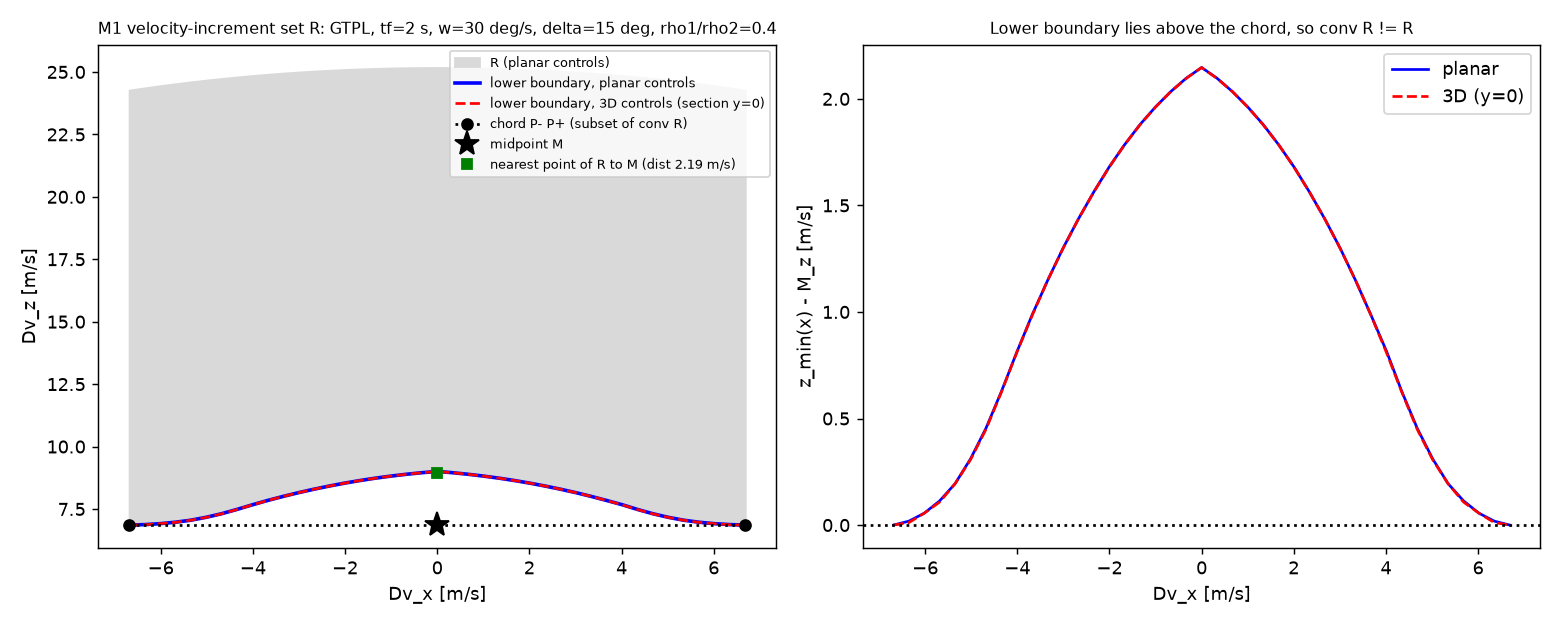
\includegraphics[width=\linewidth]{figures/t1_R_section.png}
\caption{Velocity-increment set $R$ of model M1 ($t_f=2$~s, $\omega=30^\circ$/s, $\delta=15^\circ$, $\rho_1/\rho_2=0.4$). The lower boundary
lies strictly above the chord $P_{-u}P_u$, so $M\in\conv R\setminus R$ (\cref{thm:B}). Planar and 3-D controls give the same boundary.
Numerical (inner discretization).}\label{fig:Rsection}
\end{figure}
\begin{figure}[t]\centering
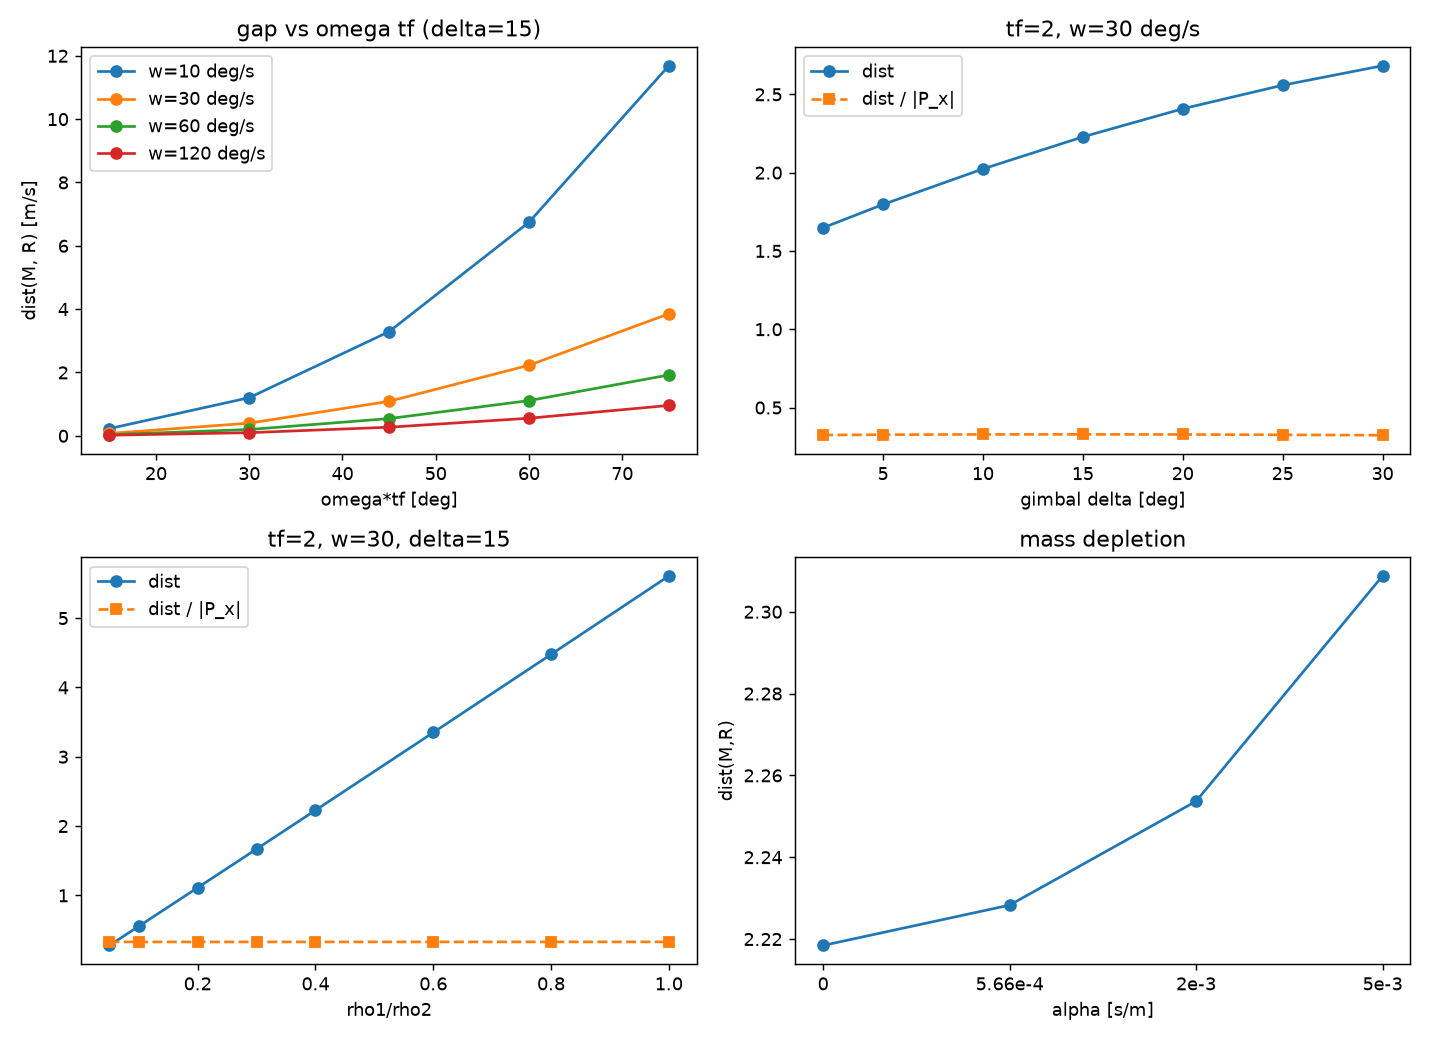
\includegraphics[width=.85\linewidth]{figures/t1_gap_sweeps.png}
\caption{Midpoint gap $\dist(M,R)$ against $\omega t_f$, $\delta$, $\rho_1/\rho_2$ and $\alpha$. The normalized gap $\dist/|P_x|$ is
flat in $\delta$ and $\rho_1/\rho_2$. Numerical.}\label{fig:gaplaw}
\end{figure}

\subsection{Beyond the proven regimes (no state constraints)}
For long horizons without a tilt cap the generalized midpoint gap grows (2.1/13.5/18.6~m/s at $t_f=2/4/8$~s), but that
regime uses inverted flight. With a $30^\circ$ tilt cap it is 1.15/1.56/0.35~m/s, shrinking as azimuthal sliding along the
cap weakens rigidity. In the tent variant the gaps are 0.66~m/s ($t_f=2$) and 6.24~m/s ($t_f=5$). For free final time the
Theorem~B witness, which starts underground, becomes reachable at a longer horizon (\cref{fig:freetf}). This is why the
free-final-time results need B$^*$ and a window. The torque-coupled TVC model M3 has nonconvex $R$ with gaps of 0.8--8~m/s
at $t_f=4$~s, and every minimizer of $\Delta v_z$ has nonzero lateral component.

\begin{figure}[t]\centering
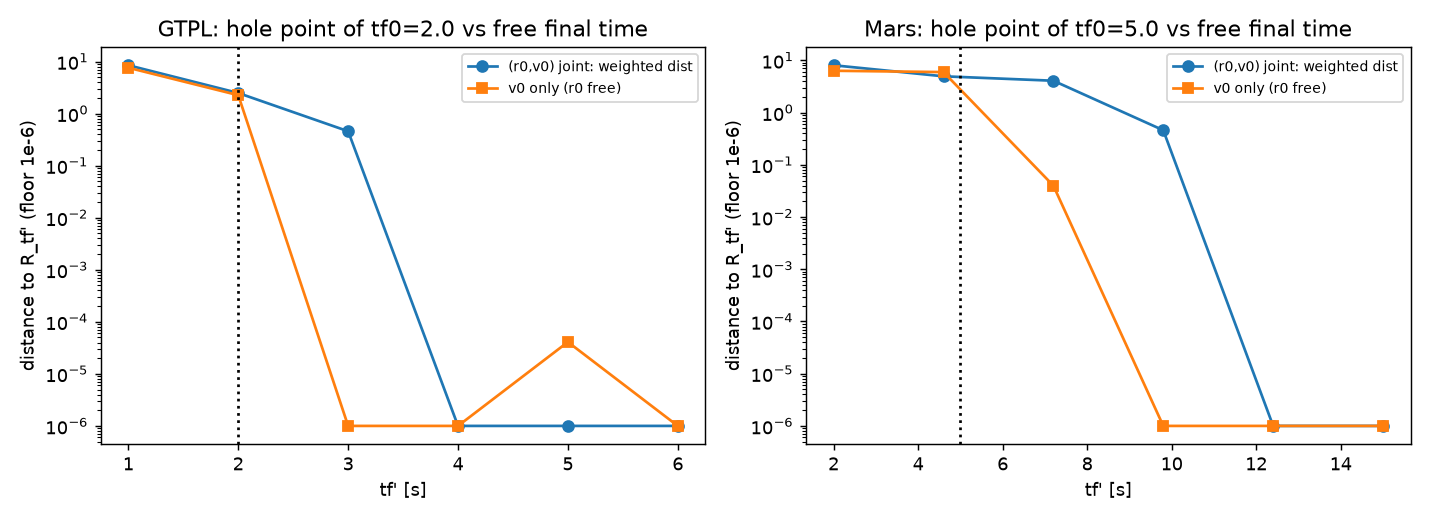
\includegraphics[width=.8\linewidth]{figures/t2_free_tf.png}
\caption{Free final time: the Theorem~B hole point at $t_f=2$~s (an underground datum) is reached at horizons $t_f'\ge4$~s. The
free-final-time obstruction therefore needs the dive-then-brake face and a compact window (\cref{cor:LS}). Numerical.}\label{fig:freetf}
\end{figure}

\subsection{With altitude constraints: the physically relevant sets}
Gaps of physically admissible data, all with $r_z(t)\ge0$ at every node, are summarized in \cref{tab:gaps}.
\begin{itemize}[leftmargin=*,itemsep=2pt]
\item \emph{B$^*$ face.} The rotation-midpoint gap is about $0.010$ (weighted m/s) at $t_f=4$~s and $0.007$ at $t_f=8$~s, stable in
$N$. That is real but tiny, roughly 0.3--0.5\% of the face's lateral velocity, consistent with \cref{rem:thin}.
\item \emph{Slice lemma (S) at dive-then-brake data.} Strict gaps of 0.016~m ($t_f=4$) and 0.009~m ($t_f=8$), with optimizers landing
1.5--2.4~m off axis. Coning narrows planar gaps by at most about 30\% (\cref{fig:slice}).
\item \emph{Face scan and the hop instance.} Among rotation-invariant vertical faces of $F^{\X}$, the pure-dive face is pinned at
$r_{0z}=0$, $v_{0z}>0$: a vehicle on the pad moving upward. Its midpoint gap is 0.65 ($t_f=4$) and 2.94 ($t_f=8$) weighted m/s,
about 65 ($t_f=4$) and 400 ($t_f=8$) times the B$^*$ gap. At pad data $r_0=0$, $v_{0,h}=0$, $t_f=4$~s, the landing-offset set $L$ is an annulus whose inner
radius grows from 0 to $4.99$~m as $v_{0z}$ goes from 7.65 to 7.90~m/s (\cref{fig:annulus}). Inside the window
$v_{0z}\in(7.727,7.917]$, landing back on the pad is infeasible while landing 0.5--8~m away is feasible. For the torque-coupled TVC
model at $v_{0z}=8.0$~m/s the pad lies 1.74~m from $L$. The \emph{rigorous} part of the hop result is an exact reduction, an
upright pad-landing limit $v_{0z}\le7.2045$ ($\alpha=0$) / $7.2833$ ($\alpha>0$), and explicit planar witnesses landing 6.58~m /
4.61~m off the pad at $v_{0z}=7.7116$ / $7.7425$. The \emph{hole} itself is not proved: quadratic and S-procedure certificates are
provably too loose here.
\item \emph{Tilt-rate-only model MT.} At the same hop data, $L$ is a full disk of radius 10.1~m. The full-direction rate limit, which
creates rigidity, is what creates the hole.
\item \emph{In-air descent.} From $r_0=(0,0,50)$~m, $v_0=(4,0,-5)$~m/s, $t_f=7$~s, the set $L$ is 104~m wide with no dent above
solver noise ($\le0.016$~m).
\item \emph{Long horizons and coning.} On the pure-dive face with a $30^\circ$ tilt cap, the 3-D slice gap falls to 0.69/0.50/0.106~m/s
at $t_f=8/12/20$~s (planar: 0.70/0.80/0.82), and at $t_f=20$~s the optimizer cones through $359^\circ$ on the cap. Coning fills
about 87\% of capped dents, but not all of them.
\item \emph{Pure TVC, upright at rest.} Full rigid body, $\pm15^\circ$ box gimbal at $100^\circ$/s from centred, mass depletion, roll free,
$r_z\ge0$, upright at rest at touchdown, face $\ell=r_{0z}+s^*v_{0z}$: the zero-lateral optimum lies below the free optimum by
$1.26\times10^{-2}$~m ($t_f=3$~s, $s^*=0.75$~s), $4.8\times10^{-3}$~m ($t_f=5$~s, $s^*=0.5$~s), $2.8\times10^{-2}$~m ($t_f=5$~s, $s^*=1$~s) and
$3.3\times10^{-2}$~m ($t_f=7$~s, $s^*=1$~s). The rigorous counterpart is \cref{thm:TVC1} (constant mass, unlimited gimbal rate; $t_f=1,2$~s uncapped, $3,5$~s capped).
\end{itemize}

\begin{table}[t]\centering\small
\caption{Size of the nonconvexity at physically admissible data ($r_z\ge0$), motivating vehicle. All entries numerical (upper bounds on true
distances, uncertified global optima) except where marked.}\label{tab:gaps}
\begin{tabular}{@{}llll@{}}\toprule
Face / instance & Model & $t_f$ [s] & Gap \\\midrule
B$^*$ face, rigorous bound (\cref{thm:Bstar}) & M1 & 7 & $\ge1.1\times10^{-5}$ (proved) \\
B$^*$ face, rotation midpoint & M1 & 4 / 8 & $\approx0.010$ / $0.007$ (weighted m/s) \\
Slice (S), dive-then-brake & M1 & 4 / 8 & 0.016 / 0.009 m in $\ell$; offsets 1.5--2.4 m \\
Pure-dive face (hop, $r_{0z}=0$) & M1 & 4 / 8 & 0.65 / 2.94 (weighted m/s) \\
Hop landing-set hole & M1 & 4 & up to 4.99 m \\
Hop landing-set hole & M3 (TVC) & 4 & 1.74 m \\
Dive-then-brake, upright at rest & PT (6-DOF) & 3 / 5 / 7 & 0.013 / 0.028 / 0.033 m \\
Same, certified (\cref{thm:TVC1}; const.\ mass) & PT (6-DOF) & 1 / 2 & $\ge9.6\times10^{-6}$ / $9.2\times10^{-5}$ m (proved) \\
Same, tilt-capped class, certified & PT (6-DOF) & 3 / 5 & $\ge4.8\times10^{-5}$ / $2.3\times10^{-6}$ m (proved) \\
In-air descent (50 m, $-5$ m/s) & M1 & 7 & none detected ($\le0.016$ m) \\\bottomrule
\end{tabular}
\end{table}

\begin{figure}[t]\centering
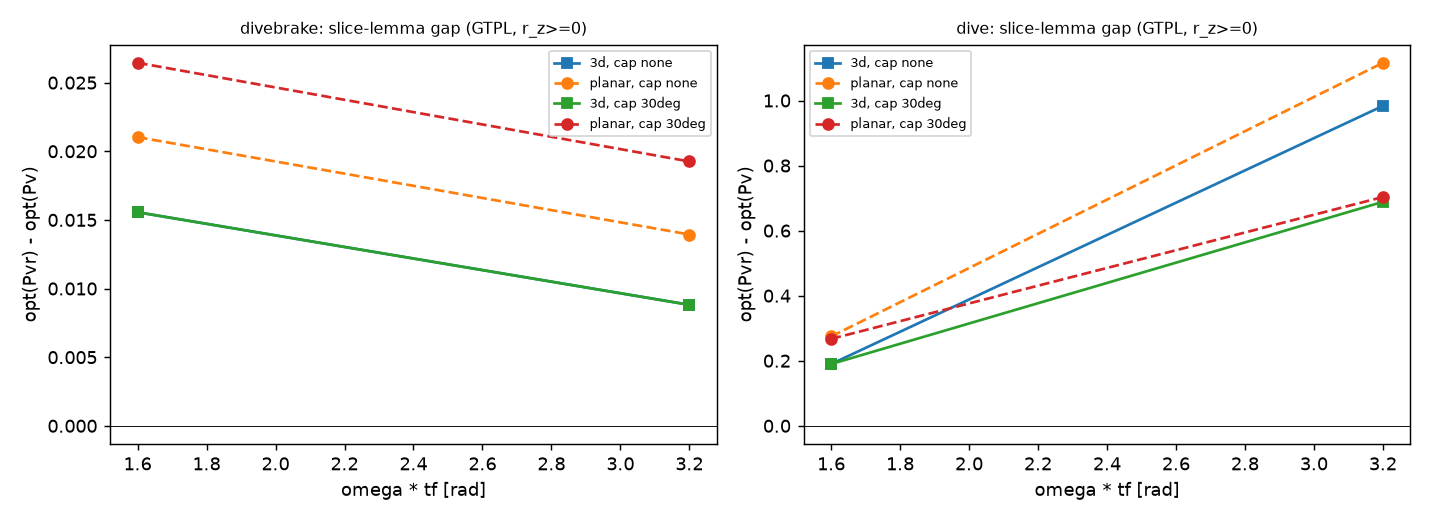
\includegraphics[width=.85\linewidth]{figures/s1_slice.png}
\caption{Slice-lemma gaps $\mathrm{opt}(P_{vr})-\mathrm{opt}(P_v)$ under $r_z\ge0$ for the dive-then-brake face (left; metres in $\ell$) and the
pure-dive face (right; m/s), planar versus 3-D (coning), with and without a $30^\circ$ tilt cap. A strictly positive gap means that the
straight-below landing is infeasible while an offset landing is feasible. Numerical.}\label{fig:slice}
\end{figure}
\begin{figure}[t]\centering
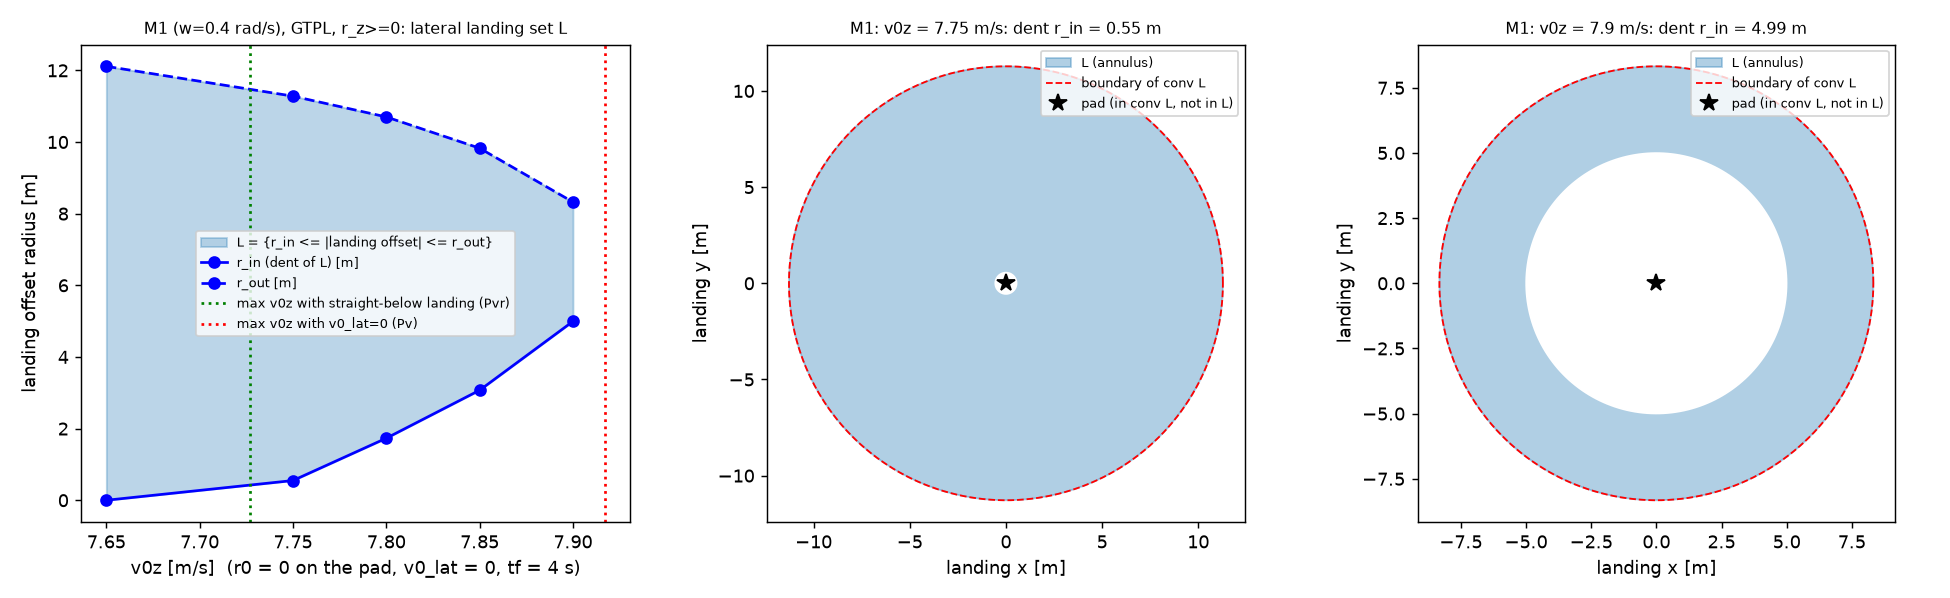
\includegraphics[width=\linewidth]{figures/s5_annulus.png}
\caption{Pad-launched hop ($r_0=0$, $v_{0,h}=0$, $t_f=4$~s, M1, $r_z\ge0$): the reachable landing-offset set $L$ is an annulus. The pad lies in
$\conv L$ but not in $L$ once $v_{0z}\gtrsim7.73$~m/s. By Theorem~D every state-linear relaxation of the minimum-landing-error problem reports
error $0$ at such data. Numerical; the hole is not certified.}\label{fig:annulus}
\end{figure}

\subsection{What 3-DOF LCvx asks of the vehicle}
The current guidance stack of the motivating vehicle solves a 3-DOF LCvx SOCP and hands only the thrust magnitude to the attitude
tracker. Its stored solutions contain thrust-direction jumps of $14.8^\circ$ within 24~ms and $180^\circ$ azimuth flips at
zero-order-hold switches. These demand roughly $10^3$~rad/s$^2$, against 1--3.5~rad/s$^2$ available. The relaxation is also not tight
on the stored minimum-throttle arc (296~N delivered against $\sigma m=400$~N), consistent with \cref{thm:CS}, which places lossiness at
minimum throttle. Together with \cref{thm:C6} (an upright body has effective cone $0$), this shows that the 5-DOF/6-DOF coupling is a
first-order issue for this vehicle, independent of the size of the nonconvexity.

% ============================================================================
\section{Practical guidance for an attitude-rate-limited TVC lander}\label{sec:practice}
% ============================================================================
\emph{This section reports an algorithm and numerical evidence. Its theorem-level ingredients are \cref{thm:C6}, \cref{thm:CU}
and the elementary claims listed below. Convergence of the outer loop is not proved.}

The theory says where the nonconvexity lives (the attitude profile, \cref{thm:CU}) and what is exactly convex (the problem for a
given attitude, \cref{thm:C6}). The planner below is built on that split. It was implemented for the motivating vehicle and
compared with the current flight guidance \pnote{solver/README.md, RESULTS.md, CLAIMS.md}.

\subsection{Planner B: attitude-aware convex guidance}
The attitude variable is the body angular acceleration $\alpha(t)$ (pitch and yaw), piecewise linear in time, so the gimbal angle
never jumps. With zero roll rate and axisymmetric inertia, the body rate is exactly linear in $\alpha$ (the gyroscopic term
vanishes), and the torque balance of \cref{thm:C6} fixes the lateral thrust, $T_x=-(J_t/L)\alpha_y$, $T_y=(J_t/L)\alpha_x$. The only
remaining control is the axial thrust $T_a(t)$.
\begin{enumerate}[leftmargin=*,itemsep=2pt]
\item \emph{Warm start.} Solve the 3-DOF problem, then fit a smooth attitude profile whose nose follows the 3-DOF thrust direction.
\item \emph{Exact inner solve.} For the fixed attitude profile, solve the SOCP in $T_a$. By \cref{thm:C6} this is the exact
problem, with no relaxation: throttle and gimbal limits become intervals in $T_a$, and the dynamics are affine in $T_a$.
\item \emph{Attitude step.} Linearize only the effect of an attitude change on the thrust direction and solve one convex
trust-region problem in $(\alpha,T_a)$. The minimum-thrust bound is replaced by its tangent plane, which is a safe inner
approximation (Cauchy--Schwarz).
\item \emph{Accept or shrink.} Re-run the exact inner solve at the new attitude. Accept if the merit (fuel plus terminal-defect and
constraint penalties) decreases sufficiently; otherwise shrink the trust region. \emph{Every accepted iterate is an exact solution
of the true dynamics for its attitude}, so the loop can be stopped at any time.
\item \emph{Certificate.} Check the returned plan, not the optimizer, against the physical limits on an $8\times$ finer grid
(throttle $400$--$1000$~N, exact gimbal angles within $\pm15^\circ$, gimbal rate $\le100^\circ$/s, throttle rate, tilt, glide slope,
touchdown defects). Then replay it open loop through a full quaternion rigid-body model, which must land within 5~cm. Fly it
only if it passes.
\end{enumerate}
Planning uses margins inside the physical limits (throttle $440$--$920$~N, gimbal $10^\circ$). Gimbal-rate limits enter as linear sufficient
conditions on node-to-node thrust changes. With $B=\omega_g T_{\rm floor}h$, $t=\tan\delta_p$, $T_z\ge T_{\rm floor}$ and $|T_x|,|T_y|\le tT_z$,
the planner imposes the \emph{pair}
\[
|\Delta T_x|+t|\Delta T_z|\le B\quad(\theta\text{ axis}),\qquad |\Delta T_y|+t|\Delta T_z|\le B\quad(\phi\text{ axis}),
\]
and the pair implies both gimbal-angle rates are at most $\omega_g$. Formalization caught an error here. The originally stated
stand-alone justification for the $\phi$ axis is false: it misses the $\dot T_x$ term, and a counterexample exists. The pair
actually imposed is nevertheless a valid sufficient condition, so no code change was needed.
\begin{todobox}[{(lean-n): Lean status of solver claims N1--N7}]
% CLAIMS: solver/CLAIMS.md N1-N7 (elementary; being formalized by lean-n)
The elementary solver claims are being formalized by [lean-n]: conservative gimbal box (N1), the gimbal-rate pair above (N2),
throttle-slew bound (N3), chord bound (N4), direction-acceleration bound (N5), linear body-rate dynamics (N6), and the 3-DOF lower
bound (N7). \emph{To fill in:} their Lean names and status.
\end{todobox}

\subsection{Results (numerical evidence)}
Comparisons: \textbf{A}, a faithful re-implementation of the flight 3-DOF LCvx; \textbf{C}, 3-DOF LCvx with SOC-representable
thrust-rate limits; \textbf{D}, IPOPT on the full quaternion rigid body (multistart); and \textbf{LB}, the 3-DOF relaxation at the same
$t_f$. Every flyable plan is feasible for the 3-DOF relaxation, so LB is a lower bound, up to its discretization, which is not
bounded rigorously.
\begin{itemize}[leftmargin=*,itemsep=2pt]
\item \emph{Open loop, 8 in-air scenarios} (\cref{fig:openloop}). Every B plan passed the certificate (replay landing within
$0.7$~mm). B is within $0.012\%$ of the best IPOPT optimum (mean $0.005\%$) and at most $0.85\%$ above LB (mean $0.34\%$), so it is
within 1\% of the 6-DOF optimum at that $t_f$. Without attitude iterations (warm start plus one inner solve), only 1 of 8 plans is
certified. C is infeasible at B's $t_f$ in all 8 scenarios; at its own minimum $t_f$ it uses $3.9$--$12.6\%$ more fuel. A's plans
are not flyable: 3 of 8 deliver 296--305~N on the ``400~N'' arc, and they demand instantaneous thrust re-pointing.
\item \emph{Closed loop} (6-DOF plant with wind, gusts, thrust noise, $5\%$ Isp error, gimbal misalignment; common tracker; 1~Hz
replans; success means touchdown $\le1$~m/s, lateral error $\le1$~m, tilt $\le5^\circ$). In-air descents (40 runs): A $28\%$, C $95\%$, B
$100\%$, with median touchdown speeds $2.42$, $0.48$ and $0.20$~m/s (\cref{fig:mcinair}). Pad hops (30 runs): A $0\%$, C $100\%$ at $+23\%$
fuel, B $97\%$ (the one failure skimmed the altitude floor; that is a formulation issue for hops). B's solver time per replan
averaged 0.2--0.4~s, with 9--60 small SOCPs per plan.
\item \emph{The impossibility, visible in practice.} On a grid of 20 pad-hop targets (launch speeds 5--7~m/s, landing offsets
0--6~m, $t_f=4$~s), the 3-DOF relaxation and the flight LCvx report ``optimal'' at all 20. Neither B nor IPOPT finds a flyable plan
at 11 of them: all 8 targets with launch speed $\ge6.5$~m/s, plus 3 targets 6~m away. B and IPOPT agree on feasibility in all 20
cells, and on fuel within $0.3\%$ where both find a plan. ``No IPOPT solution'' is not a proof of infeasibility, but this is exactly
the false-feasibility failure mode Theorem~A predicts for any uniform relaxation (\cref{cor:A}).
\end{itemize}

\begin{figure}[t]\centering
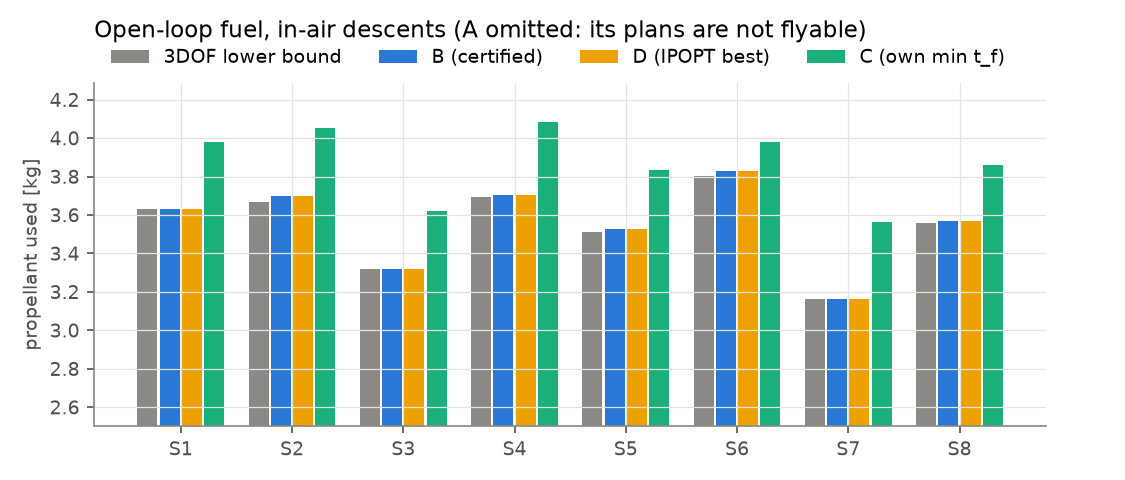
\includegraphics[width=.9\linewidth]{figures/openloop_fuel.png}
\caption{Open-loop fuel for 8 in-air descents: 3-DOF lower bound, planner B (certified), best IPOPT 6-DOF multistart, and 3-DOF with
rate limits at its own minimum $t_f$. Baseline A is omitted because its plans are not flyable. Numerical.}\label{fig:openloop}
\end{figure}
\begin{figure}[t]\centering
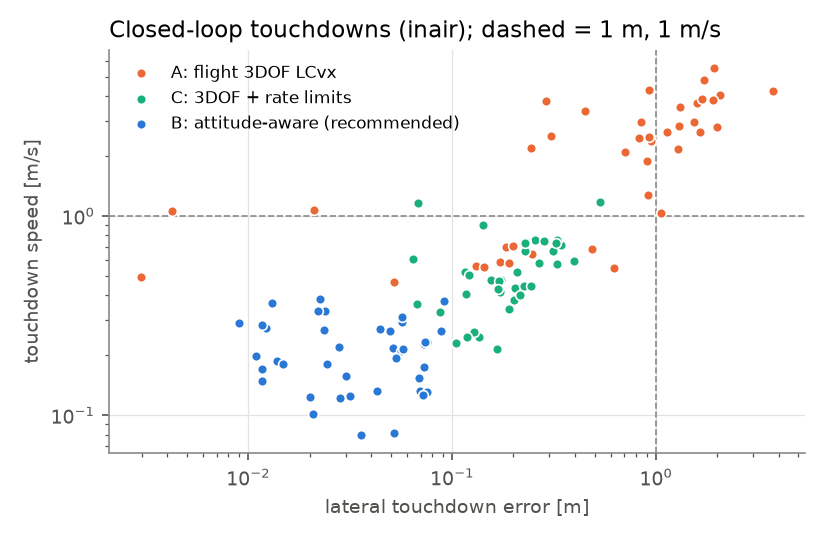
\includegraphics[width=.7\linewidth]{figures/mc_inair_touchdown.png}
\caption{Closed-loop touchdowns, 40 in-air descents per method (dashed lines: 1~m, 1~m/s). Numerical.}\label{fig:mcinair}
\end{figure}

\paragraph{What is and is not guaranteed.} By construction (\cref{thm:C6}), every accepted plan is an exact trajectory of the
planning model for its attitude. The certificate verifies flyability of each returned plan numerically, on a fine grid and by
rigid-body replay, up to floating-point integration error. Not guaranteed: convergence of the outer (SCvx-type) loop to a 6-DOF
KKT point; convergence of the mass fixed point; global optimality (only the gap to LB is bounded); and robustness to plant
mismatch, which is Monte Carlo evidence only.

% ============================================================================
\section{Machine-checked formalization}\label{sec:lean}
% ============================================================================
The obstruction is short but easy to misstate: data entry, terminal attitude, state constraints and the sign conventions of
the dive-then-brake face all matter. We therefore formalized its core in Lean~4 with Mathlib \cite{demoura2021lean4,mathlib2020}
(toolchain \texttt{v4.36.0-rc2}; project \texttt{lean/LcvxObstruction}, namespace \texttt{LcvxObstruction}). The project contains
no \texttt{sorry} and no \texttt{axiom}. For every headline theorem, \texttt{\#print axioms} reports exactly
\[
\texttt{[propext, Classical.choice, Quot.sound]},
\]
the standard axioms of classical Lean mathematics. This was checked after a full \texttt{lake build} at commit \texttt{eb2f850}.

\subsection{What is formalized}
\Cref{tab:lean} lists the formal theorems that correspond to statements in this paper. A row-by-row faithfulness map from each
Lean definition to its mathematical meaning is maintained in \texttt{lean/MODEL.md}. Its main conventions are listed next.
\begin{itemize}[leftmargin=*,itemsep=2pt]
\item $\R^3$ is \lean{EuclideanSpace \ensuremath{\mathbb{R}} (Fin 3)}. Angles are Mathlib's \lean{InnerProductGeometry.angle}. Integrals are Bochner
integrals over $[0,t_f]$.
\item \lean{UniformConvexRelaxation \ensuremath{\Theta} Y} is a convex set $C\subseteq\Theta\times Y$ for arbitrary real vector spaces $\Theta,Y$.
\lean{IsLossless F} is the feasibility form of \cref{def:lossless}(a), and \lean{IsLosslessFor J F} is the optimization (LCvx) form
(b) for an arbitrary cost $J$, including attainment.
\item \lean{AttitudeAdmissible tf \ensuremath{\omega} \ensuremath{\delta} d b} encodes M1 with variant (F): $b(0)=\ez$, unit vectors,
$\angle(b(s),b(s'))\le\omega|s-s'|$, measurable unit $d$, gimbal $\angle(d,b)\le\delta$. Pointwise constraints are imposed for every $s$,
which changes no integral. The admissible thrust accelerations form an abstract class \lean{Acc}. Theorem B assumes only
$a\ge a_1$ for a continuous $a_1>0$ (so it covers mass depletion through $a_1(s)=\rho_1/(m_0-\alpha\rho_1s)$). Theorem B$^*$ assumes a
box $a_{\min}\le a\le a_{\max}$ with constant bounds, which is exact for constant mass.
\item Positions and velocities are given in closed (Cauchy) form, $r(t)=r_0+tv_0+\tfrac{t^2}2g+\int_0^t(t-s)\,a\,d$.
\item \lean{StateLinearRelaxation} is \cref{def:statelinear} with an affine readout and a convex penalty that is nonnegative on $C$.
\end{itemize}

\begin{table}[t]\centering\footnotesize
\caption{Lean theorems corresponding to results in this paper. All compile without \texttt{sorry}; axioms
\texttt{propext}, \texttt{Classical.choice}, \texttt{Quot.sound} only.}\label{tab:lean}
\begin{tabular}{@{}>{\raggedright\arraybackslash}p{0.22\linewidth}>{\raggedright\arraybackslash}p{0.44\linewidth}>{\raggedright\arraybackslash}p{0.28\linewidth}@{}}\toprule
Paper & Lean name (file) & Formal scope \\\midrule
\Cref{thm:A}, \cref{prop:opt-feas} & \lean{theoremA}, \lean{not\_isLossless\_of\_not\_convex}, \lean{not\_isLosslessFor\_of\_not\_convex}, \lean{IsLosslessFor.isLossless} (\texttt{Abstract}) & any $\Theta,Y$, any cost \\
Spherical triangle inequality and rigidity & \lean{inner\_triangle}, \lean{inner\_triangle\_eq\_lateral}, \lean{lateral\_eq\_of\_inner\_ge} (\texttt{Sphere}) & inner-product form with equality case \\
\Cref{thm:B} (variant F) & \lean{not\_convex\_reachSet}, \lean{not\_convex\_landingSet}, \lean{no\_lossless\_relaxation\_5dof}, \lean{no\_losslessFor\_relaxation\_5dof}, \lean{landingSet\_nonempty} (\texttt{Nonconvex}, \texttt{Main}) & $\delta+\omega t_f\le\pi/2$, any continuous $a_1>0$, any $g$, no state constraints, $b(t_f)$ free \\
\Cref{thm:Bstar} (qualitative) & \lean{VStar\_not\_mem\_WSet}, \lean{witness\_mem\_glideSlope}, \lean{not\_convex\_constrainedLandingSet}, \lean{exists\_switchTime}, \lean{no\_lossless\_relaxation\_constrained\_5dof}, \lean{no\_losslessFor\_relaxation\_constrained\_5dof}, \lean{constrainedLandingSet\_nonempty} (\texttt{DiveBrake}, \texttt{Main}) & constant acceleration bounds ($\alpha=0$), $g_0<a_{\max}$, every $t_f>0$, every $\X\supseteq$ glide-slope set, $b(t_f)$ free \\
\Cref{thm:D} (abstract) & \lean{StateLinearRelaxation.convexHull\_subset}, \lean{minError\_lossy}, \lean{convex\_superset\_gap} (\texttt{TheoremD}) & abstract; concrete instance not formalized \\
\Cref{lem:LS} (abstract) & \lean{not\_lineSearch\_lossless}, \lean{symmetric\_supply}, \lean{not\_lineSearch\_lossless\_of\_symmetry} (\texttt{FreeTime}) & abstract (i)--(ii); sorry-free (commit \texttt{517f1bb}); axiom check after next full build \\\bottomrule
\end{tabular}
\end{table}

\subsection{The PMP-as-hypothesis convention}
Two external theorems appear on the positive side, and each enters only as an explicit hypothesis of the formal statement,
never as an axiom. The Pontryagin maximum principle is a structure \lean{PMPConclusion} whose fields are the adjoint equations
and the a.e.\ minimum condition of (H-PMP). Aumann's theorem enters as \lean{AumannInstance}, the single instance used in
\cref{thm:CW}. A reader can therefore check exactly which conclusions depend on which external results. The positive-side files
(\texttt{Positive/}: pointwise cap lemmas, primer geometry, \cref{thm:CS} under \lean{PMPConclusion}, discrete KKT and purification,
\cref{thm:C6} pointwise and trajectory-level convexity, \cref{thm:CW} feasibility under \lean{AumannInstance}) are summarized in
\texttt{lean/POSITIVE.md}. There the Lean form is weaker than the paper in several places, which that file lists explicitly: the
adjoint ODEs are assumed globally differentiable; C-S(2) is constant-mass only; ``$\mathrm P_0$-optimal'' is reduced to pointwise
feasibility; C-E is discrete-time; and C-W is constant-mass and unconstrained.

\begin{todobox}[{(lean, lean-s, lean-positive): formalizations still pending}]
\textbf{Not yet committed or not yet axiom-audited at the time of writing:}
\begin{itemize}[leftmargin=*,itemsep=1pt]
\item \texttt{SixDOF.lean} (\cref{thm:6kin}): \lean{not\_convex\_landingSet6}, \lean{not\_convex\_constrainedLandingSet6}. Status per [lean]: PENDING.
\item \texttt{Slice/} (lean-s): \lean{periodic\_wirtinger}, \lean{wirtinger\_scalar}, \lean{wirtinger\_lipschitz} (\cref{lem:W}); \lean{master\_inequality},
\lean{dent} (master inequality of \cref{thm:S}, constant mass); \lean{mixing}, \lean{aOpt}, \lean{no\_valueLossless\_of\_strict} (\cref{thm:Aopt}).
Lemma S itself (the witness and $0\notin\cl L$) and Theorem B$^*$ beyond the qualitative constant-mass form are not formalized.
\item \texttt{Positive/} (lean-positive): built locally, but the axiom audit output in \texttt{lean/POSITIVE.md} is a placeholder, and the files are not
yet in the root import list.
\end{itemize}
\textbf{To fill in:} move each item into \cref{tab:lean} once it is committed with a clean \texttt{\#print axioms}.
\end{todobox}

\subsection{What is not formalized}
Mass depletion in Theorem B$^*$; the terminal-attitude variants (T) and (T$'$); free final time for B$^*$ (the abstract line-search
lemma is formalized, the supply of its hypotheses from B$^*$ is not); all quantitative gaps (\cref{thm:Q}, the B$^*$ bound,
$\varepsilon$-losslessness); 6-DOF and torque models; the centre-of-percussion identity; $\rho_1=0$; the SDP results; the equivalence of
the closed-form trajectory with $r_0+\int v$ (standard Fubini). The physical scope caveat of \cref{sec:Bstar} also applies to the
formal Theorem B: its witnesses start below ground for a vehicle that cannot hover at minimum throttle. The formal Theorem B$^*$ is
the statement that covers the altitude-constrained problem.

% ============================================================================
\section{Discussion}\label{sec:discussion}
% ============================================================================

\subsection{Implications for guidance design}
\begin{enumerate}[leftmargin=*,itemsep=3pt]
\item \emph{Do not expect a single LCvx-type SOCP for attitude-rate-limited landing.} Within the class of convex programs on the
physical state with affine data entry, exactness is impossible, and this cannot be fixed by adding slacks, cuts, lifted
variables, discretization or a line search over $t_f$ (\cref{thm:A,thm:Bstar,lem:LS,thm:D}); the state-constrained core of this statement is machine-checked. Any such program, if it contains all
genuine trajectories, accepts boundary data that no flyable trajectory can land from. The flight software then has no way to
detect infeasibility from the convex program alone. The statement is about exactness. It does not say that a single SOCP cannot be
\emph{sound}; see item~3.
\item \emph{Outer attitude loop, exact convex inner problem.} The nonconvexity lies entirely in the choice of attitude profile
(\cref{thm:CU}). For a fixed attitude profile, the time-varying-cone LCvx is exact (\cref{thm:CW,thm:CS}). On a pure-TVC vehicle the
problem given the attitude is \emph{exactly} convex, with no relaxation (\cref{thm:C6}). A natural architecture is therefore an
outer search over a low-dimensional family of attitude profiles (or a sequential update of $b$) around an exact convex inner
problem. Every inner solution is then genuinely flyable, and the inner problem certifies infeasibility for the given profile.
\Cref{sec:practice} implements this architecture and evaluates it numerically. Standard successive convexification, which
linearizes the attitude together with everything else, performed as well, so the architecture's value is speed and flyable
intermediate iterates rather than better plans.
\item \emph{Or no loop at all: a sound single SOCP.} On a pure-TVC vehicle the outer loop exists only because the problem is posed
in centre-of-mass coordinates, where attitude and thrust multiply. In centre-of-percussion coordinates the dynamics are linear, and
restricting the actuator limits instead of relaxing them gives one SOCP whose plans are all flyable at every instant (\cref{thm:F}).
What it gives up is measured in \cref{sec:practiceF}: $0.1\%$ of fuel at the operating point and a few tenths of a second of
minimum flight time, concentrated in manoeuvres that tilt in order to shed thrust. Because it needs no initial trajectory, trust
region or iteration budget and solves in tens of milliseconds, it can replan at the control system's own time scale, and in our
simulations that mattered more for touchdown accuracy than the last fraction of a percent of optimality. For a new gimballed vehicle
we would start here and keep successive convexification for the manoeuvres this program refuses.
\item \emph{Count computation time.} Closed-loop comparisons that apply each plan at the instant its state was sampled favour slow
planners. With plans applied after their solver time, the planner built on \cref{thm:C6} lost 4 of 40 in-air landings it had made
before, and the lateral error of successive convexification roughly doubled.
\item \emph{Certificates.} The degree-2 SDP lift gives a rigorous lower bound on the minimum landing error and certifies
infeasibility of exact landing when positive. Its global optimality can be certified a~posteriori (rank 3, stress test), and
a~priori for coplanar targets (\cref{thm:stress,thm:coplanar}). It is a useful companion to a local or sequential solver, not a
replacement.
\item \emph{How much does it matter?} For in-air descents of a small lander, the exhibited nonconvexity is centimetre-scale, and
a sound convex program loses little in value ($0.1\%$ of fuel in \cref{sec:practiceF}). The large effects are elsewhere. First, near
lift-off (pad-launched hops) the landing set can have a metre-scale hole. Second, 3-DOF LCvx solutions ask for thrust-direction
changes far beyond the vehicle's angular acceleration (\cref{sec:numerics}). Third, on a pure-TVC vehicle the 3-DOF optimum is
essentially never exactly flyable. The ``upright body plus pointing cone'' 3-DOF model has effective cone zero.
\item \emph{Tilt-angle rate limits.} Constraining only the tilt angle from vertical, with free azimuth, removes rigidity and
appears to give convex landing sets numerically. It is not SOC-representable either, and it is not the physical constraint
of a rigid body.
\end{enumerate}

\subsection{Open problems}
\begin{enumerate}[leftmargin=*,itemsep=3pt]
\item \emph{Pure TVC, upright landing at rest, with altitude constraint.} This is the actual small-lander case. It is proved, computer-assisted and
certified in exact arithmetic, with constant mass and unlimited gimbal rate, at $t_f=1,2$~s without a tilt cap and at $t_f=3,5$~s in
the tilt-capped class (\cref{thm:TVC1}). The fully realistic model (rate-limited gimbal, mass depletion, free roll) is nonconvex
numerically at every horizon tried ($t_f=3$--$7$~s, gaps $0.5$--$3.3$~cm; a 1.7~m hole at hop data). Still open: certificates with a
gimbal-rate limit, with mass depletion, at $t_f=7$~s capped (fails by 4.8\%), for uncapped $t_f>2.3$~s (tumbling lemma), for the box
gimbal and free roll beyond $t_f=1$~s, and with free final time.
\item \emph{Rigor at realistic constants.} For our vehicle, Lemma S (hard soft landing, per instance) and the hop-instance hole
are numerical. The available quadratic, Wirtinger and S-procedure certificates are provably too loose. A two-dimensional
rigidity argument or validated branch-and-bound is needed. The $\rho_1=0$ landing-set result with altitude constraint is open at
$T/W\approx1.27$.
\item \emph{CSD2$'$.} Is the degree-2 lift exact in continuous time with fixed thrust, or for the convexified-lens and $\delta=0$
discretizations? Is there a tractable exact lift with variable throttle? (The natural degree-2 throttle lift and the separate-axis
lift CSD3 were both found lossy numerically.)
\item \emph{Minimum-fuel value-losslessness.} Does $V$ agree with its convex envelope $\conv V$ on $F$ for minimum fuel? Theorem A-opt reduces this to a convexity
question, and numerics show no violation. A positive answer would still not give an LCvx in the detection-sound sense.
\item \emph{Long horizons and coning.} At long horizons with tilt caps, coning fills most but not all of the dents. Whether
nonconvexity persists for all horizons in the tent variant, and at faces with long capped plateaus, is open.
\item \emph{Quantitative state-constrained gaps.} The rigorous B$^*$ gap ($\sim10^{-5}$~m) is far below the numerical one
($\sim10^{-2}$). A sharp quantitative version would settle how much a guidance designer actually loses.
\item \emph{The sound program of \cref{thm:F}.} (a) Formalize it; every lemma is elementary. (b) Bring the gimbal and throttle slew
limits inside the guarantee: bounds with worst-case constants are valid but too loose to be useful, and a restriction with
reference parameters, as in rows (R3)--(R5), is the natural route. (c) Bound the loss: \cref{prop:F-inc} says the program is
incomplete, and the experiments say by how much on one vehicle, but there is no theorem bounding the fuel or flight-time penalty.
(d) Remove \cref{ass:cop}: with $\varepsilon$ varying along the flight the output $y$ is no longer flat, and an extra term
$2\dot\varepsilon\dot b$ appears in $\ddot y$. (e) Is there a larger convex sound set, for instance one that allows tilting to shed
thrust in a fixed direction?
\end{enumerate}

\paragraph{Reproducibility.} \intshare{Proof notes (\texttt{math/}), the Lean project (\texttt{lean/}), numerical scripts and outputs
(\texttt{numerics/}), the planners and their benchmarks (\texttt{solver/}) and the claims registry (\texttt{comms/CLAIMS.md}) are kept
in the project repository. \texttt{paper/CLAIMS-MAP.md}
maps every theorem of this paper to its proof file, registry row and Lean name.}{The supplementary archive contains the Lean project
(\texttt{lean/}: sources, \texttt{Verify.lean}, and the notes \texttt{MODEL.md}, \texttt{POSITIVE.md}, \texttt{SLICE.md},
\texttt{SOLVER.md} and \texttt{TVC.md}, which map each Lean definition to its mathematical meaning) and the scripts, data and
derivation notes of the computer-assisted pure-TVC certificates (\texttt{certificates/}), and the code, tests and proof note of the
sound single convex program of \cref{sec:F} (\texttt{landing/}). Its \texttt{README} gives the commands that reproduce every check.}


\bibliographystyle{unsrtnat}
\bibliography{refs}

\appendix
% ============================================================================
\section{Proofs of Theorems B and Q}\label{app:B}
% ============================================================================
\intshare{Adapted from project note \texttt{math/02} \S\S1--5. }{}Throughout, M1 of \cref{sec:models}.

\begin{lemma}[Spherical triangle inequality, inner-product form]\label{lem:tri}
% CLAIMS: P-B (lemma) | Lean: inner_triangle, inner_triangle_eq_lateral (Sphere.lean)
Let $x,y,z\in\Sph$, $\alpha,\beta\in[0,\pi]$, $\alpha+\beta\le\pi$, $\ip xy\ge\cos\alpha$, $\ip yz\ge\cos\beta$. Then (a)
$\ip xz\ge\cos(\alpha+\beta)$. (b) If $\ip xz=\cos(\alpha+\beta)$ and $\alpha+\beta<\pi$, then $\ip xy=\cos\alpha$, $\ip yz=\cos\beta$, and,
if $\beta\in(0,\pi)$, $x=\cos\alpha\,y-\frac{\sin\alpha}{\sin\beta}(z-\cos\beta\,y)$.\Slean
\end{lemma}
\begin{proof}
Write $p=\ip xy=\cos a$, $q=\ip yz=\cos c$ with $a\le\alpha$, $c\le\beta$, and $x'=x-py$, $z'=z-qy$, both orthogonal to $y$. Then
$\ip xz=pq+\ip{x'}{z'}\ge\cos a\cos c-\sin a\sin c=\cos(a+c)\ge\cos(\alpha+\beta)$. Equality forces $a=\alpha$, $c=\beta$ (strict
monotonicity of $\cos$ on $[0,\pi]$) and $\ip{x'}{z'}=-\norm{x'}\norm{z'}$, i.e.\ $x'$ is a nonpositive multiple of $z'$.
\end{proof}
\begin{corollary}[Extremal thrust direction]\label{cor:extremal}
If $\ip db\ge\cos\delta$, $\ip b\ez\ge\cos\varphi$, $\varphi\in(0,\pi)$, $\delta+\varphi<\pi$, then $d_z\ge\cos(\delta+\varphi)$. Equality implies
$b=\cos\varphi\,\ez+\sin\varphi\,u$ for a horizontal unit $u$ and $d=\cos(\delta+\varphi)\ez+\sin(\delta+\varphi)u$.
\end{corollary}
\begin{lemma}[Rigidity]\label{lem:rigid}
% CLAIMS: P-B (lemma) | Lean: lateral_eq_of_inner_ge (Sphere.lean)
If $b(s)=\cos\psi\,\ez+\sin\psi\,u$, $b(s')=\cos\psi'\,\ez+\sin\psi'\,u'$ with $\psi,\psi'\in(0,\pi)$, $u,u'$ horizontal unit vectors, and
$\ip{b(s)}{b(s')}\ge\cos(\psi-\psi')$, then $u=u'$.\Slean
\end{lemma}
\begin{proof}
$\ip{b(s)}{b(s')}-\cos(\psi-\psi')=\sin\psi\sin\psi'(\ip u{u'}-1)\ge0$ forces $\ip u{u'}=1$.
\end{proof}

\begin{proof}[Proof of \cref{thm:B}]
The extreme arcs \eqref{eq:arcs} are admissible: $\ip{b_u(s)}{b_u(s')}=\cos(\varphi(s)-\varphi(s'))$ and $\varphi$ is $\omega$-Lipschitz; the
gimbal angle is $\delta$; $a=a_1$ at constant minimum throttle. So $P_{\pm u}\in R$ and $M\in\conv R$. Suppose $M=\int a\,d$ for an
admissible $(T,d,b)$. In both variants $\omega t_f\le\pi$ and $0\le\delta+\varphi\le\pi/2$.

\emph{Step 1.} \eqref{eq:AL} with $s'=0$ (and $s'=t_f$ in variant T) gives $b_z(s)\ge\cos\varphi(s)$. By \cref{lem:tri}(a),
$d_z\ge\cos(\delta+\varphi)\ge0$, and with $a\ge a_1$, $a\,d_z\ge a_1d_z\ge a_1\cos(\delta+\varphi)$ a.e.
\emph{Step 2.} Integrating, $M_z\ge\int a_1\cos(\delta+\varphi)=M_z$, so the nonnegative integrand $a\,d_z-a_1\cos(\delta+\varphi)$ vanishes a.e.
Since $a_1>0$, $d_z=\cos(\delta+\varphi)$ a.e.
\emph{Step 3.} By \cref{cor:extremal}, for a.e.\ $s\in(0,t_f)$, $b_z(s)=\cos\varphi(s)$ and
$d(s)=\cos(\delta+\varphi)\ez+\sin(\delta+\varphi)u(s)$, where $u(s)$ is the azimuth of $b(s)$.
\emph{Step 4.} $b_z-\cos\varphi$ is continuous and vanishes a.e., hence everywhere, so $u(\cdot)$ is defined and continuous on $(0,t_f)$.
\emph{Step 5.} In variant F, for $0<s<s'$, \eqref{eq:AL} gives $\ip{b(s)}{b(s')}\ge\cos(\varphi(s')-\varphi(s))$, and \cref{lem:rigid} gives
$u(s)=u(s')$. In variant T apply this on $(0,t_f/2]$ and on $[t_f/2,t_f)$ and chain through $t_f/2$. So $u\equiv u_0$.
\emph{Step 6.} $I_h=(\int a\sin(\delta+\varphi))u_0$ with coefficient $\ge\int a_1\sin(\delta+\varphi)>0$, contradicting $M_h=0$.
Nonconvexity of $\Ft$ follows from \cref{lem:reduction}, and impossibility from \cref{thm:A}.
\end{proof}

\begin{lemma}[Support bound]\label{lem:support}
For any admissible control (no boundary condition on $b$ needed) and $\tau$ with $\delta+\omega\max(\tau,t_f-\tau)\le\pi/2$,
$\norm I\ge\ip{I}{b(\tau)}\ge G(\tau)=\int_0^{t_f}a_1(s)\cos(\delta+\omega|s-\tau|)\,ds$.
\end{lemma}
\begin{proof}
\eqref{eq:AL} gives $\ip{b(s)}{b(\tau)}\ge\cos(\omega|s-\tau|)$, and \cref{lem:tri}(a) gives $\ip{d(s)}{b(\tau)}\ge\cos(\delta+\omega|s-\tau|)\ge0$.
Multiply by $a\ge a_1$ and integrate.
\end{proof}

\begin{proof}[Proof of \cref{thm:Q}]
For $I\in R$, $\norm{I-M}\ge\norm I-\norm M\ge G(t_f/2)-M_z$ by \cref{lem:support}. With $c(x)=\cos(\delta+\omega x)$, strictly decreasing on
$[0,t_f]$, put $h(s)=c(|s-t_f/2|)-c(s)$. Then $h\ge0$ for $s\ge t_f/4$ and $h<0$ for $s<t_f/4$. Since $a_1$ is nondecreasing,
$(a_1(s)-a_1(t_f/4))h(s)\ge0$, so $G(t_f/2)-M_z=\int a_1h\ge a_1(t_f/4)\int h$. A direct computation, using
$\sin x+\sin(x+2k)=2\sin(x+k)\cos k$, gives
$\int_0^{t_f}h=\frac4\omega\sin(\delta+\frac{\omega t_f}2)\sin^2\frac{\omega t_f}4$. The sign condition holds if $\delta+\omega t_f\le\pi/2$
(nonnegative integrand), or if $\alpha=0$, where $M_z=\frac{a_1}\omega(\sin(\delta+\omega t_f)-\sin\delta)\ge0$. The relaxation statement is
\cref{cor:A}(ii) together with \cref{lem:reduction}.
\end{proof}

% ============================================================================
\section{Proof of Theorem B$^*$}\label{app:Bstar}
% ============================================================================
\intshare{Adapted from project note \texttt{math/02} \S10, which survived adversarial review (\texttt{math/01}). }{}Notation:
$a_{10}=\rho_1/m_0$, $a_{\max}=\rho_2/(m_0-\alpha\rho_2t_f)$, $A_b=\rho_2/m_0-g_0$, $w(s)=s-s^*$. For a control $c$ put
$W(c)=\int w\,a\,d$, $X(c)=\int_0^{s^*}(s^*-s)a\,d$, $B(c)=\int_{s^*}^{t_f}(s-s^*)a\,d$, so $W=-X+B$. By \eqref{eq:lambda},
$\Lambda(\theta)=W(c)+\kappa\ez$ with $\kappa=g_0t_f(s^*-t_f/2)$, for any control $c$ landing from $\theta$.

\begin{proof}[Proof of \cref{thm:Bstar} (qualitative part)]
\emph{Step 1 (direction bound for a fixed throttle).} Fix $T$, hence $a=a_T>0$. On $[0,s^*]$, $b_z\ge\cos\omega s$ and
$\delta+\omega s\le2\delta<\pi$, so $d_z\ge\cos(\delta+\omega s)$. On $(s^*,t_f]$, $d_z\le1$. Since $w<0$ before $s^*$ and $w>0$ after,
\[
W_z(c)\le V(T):=-\int_0^{s^*}(s^*-s)a_T\cos(\delta+\omega s)\,ds+\int_{s^*}^{t_f}(s-s^*)a_T\,ds .
\]
\emph{Step 2 (attained for every $T$).} The dive-then-brake control $c^T_u$ uses $b=\cos(\omega s)\ez+\sin(\omega s)u$ and
$d=\cos(\delta+\omega s)\ez+\sin(\delta+\omega s)u$ on $[0,s^*]$, then $b\equiv b(s^*)$ and $d=\ez$. It is admissible, because by (S1)
$\angle(\ez,b(s^*))=\omega s^*\le\delta$. In variant (T$'$), return $b$ meridionally to $\ez$ on $[s^*,2s^*]$. The gimbal angle stays $\le\delta$.
\emph{Step 3 (late throttle).} Replacing $T$ by $\rho_2$ on $(s^*,t_f]$ leaves $a$ unchanged before $s^*$ and does not decrease it after. So
$V(T)\le V(T^\sharp)$, strictly unless $T=\rho_2$ a.e.\ late.
\emph{Step 4 (outer maximum).} $V^*=\sup_TV(T)$ is attained, explicitly for $\alpha=0$ ($T^*=\rho_1$ then $\rho_2$), and for $\alpha>0$ by
weak-$*$ compactness of the throttle set and weak-$*$ continuity of $V$.
\emph{Step 5 (state constraints).} On the brake $d=\ez$, so $v_h=r_h=0$ there and $\dot v_z\ge A_b$. Hence $v_z(t)\le-A_b(t_f-t)$ and
$r_z(t)\ge\tfrac12A_b(t_f-t)^2$. On the dive $\dot v_z\ge-g_0$, so $v_z<0$ by (S2). Thus $r_z$ is decreasing, hence positive before
$t_f$. Laterally $\norm{r_h}\le\tfrac12a_{\max}s^{*2}$, and (S3) gives the glide slope. By rotation invariance, $R_\pi\theta^*$ is landed by
$c^{T^*}_{-u}$.
\emph{Step 6 (midpoint infeasible).} $\Lambda(\theta_m)=(V^*+\kappa)\ez$. If $\theta_m\in\Ft$ via $c$, then $V^*=W_z(c)\le V(T)\le V^*$, so all
inequalities are equalities a.e. On the dive, $d_z=\cos(\delta+\omega s)$, so \cref{cor:extremal,lem:rigid} give a constant azimuth $u_0$. On
the brake, $d=\ez$. Then $W_h(c)=-(\int_0^{s^*}(s^*-s)a_T\sin(\delta+\omega s))u_0\ne0$, contradicting $W_h(c)=\Lambda_h(\theta_m)=0$.
\end{proof}

\begin{proof}[Proof of the quantitative bound ($\delta\le\pi/4$)]
Let $c$ land from $\theta\in\Ft$ and put $\eta=V^*-W_z(c)\ge\eta_{dive}+\eta_{brake}$, the deficits relative to Step 1. Let $\tau=\vartheta s^*$ with
$\vartheta=a_{10}\sin\delta/(4a_{\max})\le\tfrac14$, and $c_\tau=b(\tau)$, of tilt $\beta\le\omega\tau$.
(i) As in \cref{lem:support}, $\ip{X}{c_\tau}\ge G(T):=\int_0^{s^*}(s^*-s)a_T\cos(\delta+\omega|s-\tau|)$, since $\delta+\omega s^*\le\pi/2$.
(ii) With $c_\tau=\cos\beta\,\ez+\sin\beta\,n$: $\sin\beta\norm{X_h}\ge G-X_z\ge G-Z_0-\eta_{dive}$, where $Z_0=\int_0^{s^*}(s^*-s)a_T\cos(\delta+\omega s)$.
(iii) The mean value theorem gives $G-Z_0\ge\omega\tau\gamma_X$, using $(1-\vartheta)^2-\tfrac14\ge\tfrac5{16}$.
(iv) Since $\sin\beta\le\omega\tau$: $\norm{X_h}\ge\gamma_X-c_1\eta_{dive}$ with $c_1=1/(\omega\tau)$.
(v) $\norm{d_h}\le\sqrt{2(1-d_z)}$ and Cauchy--Schwarz give $\norm{B_h}\le\sqrt{2W_b\eta}$.
(vi) $\norm{\Lambda(\theta)-\Lambda(\theta_m)}^2=\norm{W_h}^2+\eta^2$ and $\norm{W_h}\ge\gamma_X-c_1\eta-\sqrt{2W_b\eta}$, so
$\norm{\Lambda(\theta-\theta_m)}\ge\eta_0$. Finally, $\norm{\Lambda}=\sqrt{1+s^{*2}}$.
\end{proof}

\begin{proof}[Proof of the free-final-time window variant]
Take $W=[t_a,t_b]$ with $s^*<t_a$, (S1)--(S3) at $t_a$ with $a_{\max}$ evaluated at $t_b$ (they are monotone in $t_f$), and, under a
dry-mass constraint, $m_0-\alpha\rho_2t_b\ge m_{dry}$ so that the full-throttle brake of every witness is fuel-feasible.
$\ell^*(t)=\sup_{F_t}\ell=V^*_t+\kappa(t)$ is continuous in $t$, so it attains its maximum on $[t_a,t_b]$ at some $t^\circ$. If the union were
convex, $\theta_m(t^\circ)\in F_{t'}$ for some $t'$ with $\ell(\theta_m)\ge\ell^*(t')$. Then $\theta_m$ would be a maximizer at horizon $t'$, and
Step 6 at that horizon forces $\Lambda_h\ne0$. Note that $\Lambda$ does not depend on the horizon.
\end{proof}

% ============================================================================
\section{Proof of Theorem S (Lemma S in a regime)}\label{app:S}
% ============================================================================
\intshare{Adapted from project note \texttt{math/07}, which survived adversarial review (\texttt{math/01} \S9). }{}Model M1, $b(t_f)$ free, $T:=t_f$,
$\Omega=\omega T$, $\tau(s)=\delta+\omega s$, $\bar\tau=\delta+\Omega$, $a_{10}=\rho_1/m_0$, $a_2=\rho_2/(m_0-\alpha\rho_2T)$,
$\varepsilon_m=a_1(T)/a_{10}-1$. The lateral force is $F=a\,d_h$, and the \emph{gain} of a control is $\int a_1-I_z$, the vertical
impulse wasted relative to upright minimum throttle. $P$ is the $L^2((0,T);\R^2)$ projection onto affine functions. It depends
only on the moments $m(F)=(\int F,\int sF)$, and $\pi_m$ denotes the affine function with moments $m$. In particular
$\norm{\pi_{(0,q)}}^2=12|q|^2/T^3$.

\paragraph{Landing from vertical data.} From $\zeta=(h\ez,v_{0z}\ez)$ a trajectory lands at $(p,0)$ with $v(T)=0$ iff $I_h=0$,
$I_z=g_0T-v_{0z}$, $\int sF=-p$ and $J_z$ is fixed by $\zeta$. Hence \emph{every trajectory from $\zeta$ has the same gain}, and
$m(F)=(0,-p)$.

\begin{proof}[Proof of \cref{lem:W}]
Let $\tilde f=f-f(0)-\tfrac sT(f(T)-f(0))$. Then $f-Pf=\tilde f-P\tilde f$, and $\norm{\tilde f-P\tilde f}\le\norm{\tilde f-\bar{\tilde f}}$ for the mean
$\bar{\tilde f}$. Since $\tilde f(0)=\tilde f(T)=0$, $\tilde f$ extends periodically, and the periodic Wirtinger inequality (Parseval) gives
$\norm{\tilde f-\bar{\tilde f}}^2\le(T/2\pi)^2\norm{\dot{\tilde f}}^2=(T/2\pi)^2(\norm{\dot f}^2-|f(T)-f(0)|^2/T)$. All steps are componentwise.
\end{proof}

\paragraph{Master inequality.} With $c_0=1/(1+\cos\delta)$, $\delta_e=2\sin(\delta/2)+\varepsilon_m\sin\bar\tau$,
$E_4=a_{10}(1+\varepsilon_m)^2\int_0^T(\frac1{1+\cos\tau(s)}-c_0)\sin^2\tau(s)\,ds$, $B=a_{10}c_0T(\frac\Omega{2\pi}+\delta_e)^2+E_4$,
$A'=c_0/a_{10}$, $\kappa_0=\cos\bar\tau/((a_2-a_{10})\sin^2\bar\tau)$ and $C_m=A'\kappa_0/(\kappa_0-A')$ ($C_m=A'$ if $\rho_1=\rho_2$):
\begin{proposition}[Master inequality {\pnote{math/07, Prop.~M}}]\label{prop:master}
% CLAIMS: S-M (CONFIRMED by verify-imp; FORMALIZED for constant mass) | Lean: master_inequality (variant (c), constant mass), master_inequality_fixed, dent (Slice/Master.lean; PENDING)
If $\bar\tau<\pi/2$ and $\kappa_0>A'$, every admissible M1 trajectory (any 3-D attitude path, throttle, $\alpha\ge0$) satisfies
$\mathrm{gain}\le B+C_m\norm{\pi_{m(F)}}^2$.\Sproved\ \Sleanpart{constant mass, variant with constant $\bar c(T)$}
\end{proposition}
\begin{proof}[Proof sketch]
(1) A pointwise majorant $-a\,d_z\le-a_1+a_1\bar c|d_h|^2-(a-a_1)\cos\tau$ with $\bar c=1/(1+\cos\tau)$ splits off the throttle surplus
$K=(a-a_1)d_h$, which costs at least $\kappa_0\norm K^2$. (2) Normalize the mass. (3) Eliminate $K$ through its projection
($PK=\pi_m-a_{10}Pv$) by maximizing a concave quadratic. (4) The only nonconvex step bounds the non-affine part of the lateral tilt
$\beta=b_h$, which is $\omega$-Lipschitz, by \cref{lem:W}: $\norm{P^\perp\beta}\le\omega T^{3/2}/(2\pi)$. The gimbal and mass corrections are
bounded pointwise by $\delta_e$.
\end{proof}

\paragraph{Witness.} A planar single-crossing S-turn at minimum throttle: tilt $\varphi(s)=\omega s$ for $s\le t_1$ and $\omega(2t_1-s)$
after, the thrust deflected outward by $\delta$ ($\chi=\varphi+\delta\,\mathrm{sgn}\,\varphi$), and $t_1$ chosen by the intermediate value
theorem so that $\int a_1\sin\chi=0$ (so $I_h=0$). Its mean-square lateral tilt is $(3\sqrt2-4)/6\cdot\Omega^2\approx0.0404\,\Omega^2$ in the
small-angle limit ($t_1=(1-1/\sqrt2)T$). This exceeds the Wirtinger cap $\Omega^2/(4\pi^2)\approx0.0253\,\Omega^2$. The witness does not return to
zero tilt, which is why it beats every path whose two lateral moments vanish.

\begin{proof}[Proof of \cref{thm:S}]
(1) Along the witness $\dot v_z=a_1\cos\chi-g_0>0$ by (S1), so $v_z<0$ on $[0,T)$ and $r_z>0$ before $T$. Rotations about $\ez$ preserve
$\zeta_w$, so $L(\zeta_w)$ contains the circle $|p|=|p_w|$. (2) Every trajectory from $\zeta_w$ landing at $(p,0)$ has gain $\mathrm{gain}_w$
and $m(F)=(0,-p)$, so \cref{prop:master} gives $\mathrm{gain}_w\le B+12C_m|p|^2/T^3$, i.e.\ $|p|\ge r_S$. (3) Apply \cref{thm:D} with
$\varphi(x)=\norm{x_r}+\iota_{\{x_v=0\}}(x)$; since $0\in\conv L(\zeta_w)$, the relaxed value is $0$.
\end{proof}

\begin{table}[h]\centering\small
\caption{Certified instances of \cref{thm:S} for a demonstration vehicle ($m_0=100$~kg, $\rho_1=1200$~N, $\rho_2=2500$~N, $\alpha=0$)\intshare{,
from \texttt{math/07} \S4}{}.}\label{tab:S}
\begin{tabular}{@{}lccccc@{}}\toprule
$\delta$ & $T$ [s] & $\Omega$ [rad] & margin $M$ [m/s] & dent $r_S$ [m] & witness offset $|p_w|$ [m]\\\midrule
$0$ & 2 & 0.40 & $1.39\times10^{-2}$ & 0.45 & 0.94\\
$0$ & 4 & 0.40 & $2.78\times10^{-2}$ & 1.80 & 3.74\\
$5^\circ$ & 2 & 0.30 & $1.57\times10^{-2}$ & 0.48 & 1.79\\
$10^\circ$ & 2 & 0.20 & $1.06\times10^{-2}$ & 0.39 & 2.59\\
$10^\circ$ & 4 & 0.20 & $2.11\times10^{-2}$ & 1.57 & 10.38\\\bottomrule
\end{tabular}
\end{table}
For $\delta>0$ the certified range of $\Omega$ has a positive lower end: as $\Omega\to0$ at fixed $\delta$, $\mathrm{gain}_w\to a_{10}T(1-\cos\delta)$
while $B\to a_{10}T\cdot2\sin^2(\delta/2)\cdot2/(1+\cos\delta)$, which is larger, so $M<0$. At $T=2$~s the certified ranges are $(0,0.55]$
($\delta=0$), $[0.004,0.46]$ ($5^\circ$), $[0.009,0.42]$ ($7^\circ$), $[0.038,0.34]$ ($10^\circ$) and $[0.070,0.27]$ ($12^\circ$) (independent \intshare{referee}{re-}
computation). All rows of \cref{tab:S} lie inside them.
With $\alpha=5.66\times10^{-4}$ the $\delta=5^\circ$ row fails narrowly, because $\varepsilon_m$ enters $\delta_e$ linearly. That is a weakness of the constants,
not of the geometry. For $\delta\ge15^\circ$ the analytic constants do not certify; a discretized S-procedure SDP suggests $\delta=15^\circ$
holds with an 8\% margin (numerical).

% ============================================================================
\section{Further proof sketches}\label{app:other}
% ============================================================================

\subsection{Theorem P0-F ($\rho_1=0$)}
Adapted from \texttt{math/possibility-rho0} \S2. Set $\rho_1=0$, $\alpha=0$, $a_2=\rho_2/m_0$, units $\omega=a_2=1$, $T=\omega t_f$. For fixed $b$ the
pointwise control set $U(b)=\{u:
orm u\le a_2,\ \ip ub\ge
orm u\cos\delta\}$ (convex, containing $0$) has support function
$a_2\norm p\,c(\angle(p,b))$ with $c(x)=1$ for $x\le\delta$, $\cos(x-\delta)$ for $\delta\le x\le\delta+\pi/2$, and $0$ beyond. $K$ is compact and
star-shaped about $0$, so it is convex iff every exposed face lies in $K$.

Take $\hat p=(\cos\delta,0,-\sin\delta)$ and $\sigma\in(0,t_f)$, primer $p(s)=(s-\sigma)\hat p$, face functional
$\ell_\sigma=\ip{\hat p}{\int(s-\sigma)a\,d}=\ip{\hat p}{r_0+\sigma v_0}+\text{const}$. With $\beta=\phi_0-\angle(\hat p,b)$ (an $\omega$-Lipschitz tilt toward
$\hat p$, $\beta(0)=0$) one has $\ell_\sigma\le a_2P[\beta]$ for an explicit integral $P$, with equality along great circles through $\ez$ and
$\hat p$. For fixed $\beta^*=\beta(\sigma)$ the optimal profile is the lower envelope before $\sigma$ and the upper envelope after, so
$h_K=a_2\max_{\beta^*}V(\beta^*)$ with $V=E+L_t$. Here $E$ is nonincreasing (strictly on $[-T,0]$, because $T<\pi/2-2\delta$), and $L_t$ vanishes iff
$\beta^*\le-\tau$, $\tau=T-\sigma$. Let $A(\sigma)=E(-\sigma)$ and $B(\sigma)=\max_{[-\tau,\sigma]}V$. At $\sigma=T$, $B<A$. At $\sigma=T/2=h$,
$A-V(h)\le-f(h)$ with $f(h)=\sin2h-h\cos2h+\sin h-2h\ge h^3(\tfrac12-\tfrac23h^2)>0$, so $B>A$. Hence there is a tie $\sigma_c\in(T/2,T)$. The
two groups of maximizers are compact, disjoint, and separated by $\ip{\hat p}{I}$: the left group coasts late, while the right group thrusts
late and less early. A convex face cannot be a disjoint union of two nonempty compact sets, because convex sets are connected. \qed

\subsection{Theorem C-W (fixed attitude)}
Adapted from \texttt{math/04} \S3. The extreme points of the cap $K_\Gamma(b)$ are exactly its spherical part
$S_\Gamma(b)=\{\norm T=\Gamma,\ \angle(T,b)\le\delta\}$, and $K_\Gamma=\conv S_\Gamma$ (Krein--Milman; Lean: \lean{extremePoints\_cap},
\lean{cap\_subset\_closure\_convexHull\_sCap}). On each subinterval between prescribed nodes, the state increment is
$\int\Psi_k(s)T(s)/m(s)\,ds$ with $\Psi_k$ of full column rank and $m$ fixed by $\Gamma$. Aumann's theorem applied to the multifunction
$\Psi_kS_\Gamma(b)/m$ yields a measurable lossless selection with the same increment. Concatenation over subintervals preserves the state at
every node. \qed

\subsection{Theorem C-6 (pure TVC given attitude)}
With zero roll rate the angular momentum is $J_\perp b\times\dot b$, and Euler's equation reads $J_\perp b\times\ddot b=L\,T\times b$. Splitting $T$ and $\ddot b$
into components along and orthogonal to $b$ gives $\Pi_bT=-k\Pi_b\ddot b$. So $T=T_ab+F$ with $F$ determined by $b$. The gimbal condition becomes
$\varkappa\le T_a\tan\delta$, and the throttle condition becomes $\rho_1^2\le T_a^2+\varkappa^2\le\rho_2^2$. Both are intervals in $T_a$. The dynamics are
affine in $T_a$ for fixed $b$, and the fuel integrand $\norm{(T_a,\varkappa)}$ is convex. \qed


\end{document}
